\documentclass[
    a4paper, % Stock and paper size.
    9pt, % Type size.
    %article,
    oneside, 
    onecolumn, % Only one column of text on a page.
    openright, % Each chapter will start on a recto page.
    % openleft, % Each chapter will start on a verso page.
    % openany, % A chapter may start on either a recto or verso page.
    ]{memoir}
\usepackage[utf8]{inputenc}
\usepackage[T1]{fontenc}
\usepackage{lmodern}
\usepackage[final]{microtype}
\usepackage[dvips]{graphicx}
\usepackage{xcolor}
\usepackage{pgfplots}
\usepackage{tikz}
\usepgfplotslibrary{groupplots}
\usepackage{epstopdf}
\usepackage{multirow}
\usepackage{multicol}
\usepackage[ruled,vlined]{algorithm2e}
\usepackage{placeins}
\usepackage{amsfonts} 

\usetikzlibrary{patterns}
\usetikzlibrary{positioning}
\usepackage[mode=buildnew]{standalone}

\graphicspath{{automated_graphs/}{.}{images/}{images/morphmask_denoise2_erode2_MyoSegmenTUM_043}}


\usetikzlibrary{calc}
\usepackage{caption}
%\usepackage{times}

% Comment in final version
\usepackage{todonotes}
\usepackage{soul}
\usepackage{pdfpages}

%\usepackage[margincaption,outercaption,ragged,wide]{sidecap}
\usepackage[margincaption,ragged]{sidecap}
\sidecaptionvpos{figure}{t} 
\sidecaptionvpos{table}{t}

\usepackage[
breaklinks=true,colorlinks=true,
%linkcolor=blue,urlcolor=blue,citecolor=blue,% PDF VIEW
linkcolor=black,urlcolor=black,citecolor=black,% PRINT
bookmarks=true,bookmarksopenlevel=2]{hyperref}

\usepackage{geometry}
% PDF VIEW
% \geometry{total={210mm,297mm},
% left=25mm,right=25mm,%
% bindingoffset=0mm, top=25mm,bottom=25mm}
% PRINT
% \geometry{total={210mm,297mm},left=20mm,right=50mm,bindingoffset=10mm, top=25mm,bottom=25mm}

% Code from https://tex.stackexchange.com/questions/275565/tufte-layout-in-painless-memoir

% Start code

% MEMOIR LAYOUT
\setlength{\baselineskip}{14pt}
\setlength{\normalbaselineskip}{14pt}

% GEOMETRY
\settrims{0pt}{0pt}
\settypeblocksize{49\baselineskip}{107mm}{*}
\setlrmargins{20.0mm}{*}{*} % 24.8 mm
\setulmargins{20.0mm}{*}{*} % 27.4 mm
\setheadfoot{\baselineskip}{\baselineskip}
\setheaderspaces{*}{2\baselineskip}{*}
\setmarginnotes{8.2mm}{49.4mm}{\onelineskip}
\checkandfixthelayout


% TEXT
% ragged2e provides ragged justification with hyphenation
\RequirePackage{ragged2e}
\AtBeginDocument{\RaggedRight}
\setmpjustification{\RaggedLeft}{\RaggedRight}
\setlength{\RaggedRightParindent}{1.0pc}
\setlength{\parindent}{1pc}
\setlength{\parskip}{0pt}
% linespacing ~ 14pt
\linespread{1.17}

% text styling of all side footnotes
\renewcommand{\footnotesize}{\fontsize{8pt}{10pt}\selectfont}
\renewcommand{\foottextfont}{\footnotesize}
% styling and placement of mark
\footmarkstyle{{#1. }}
\setlength{\footmarkwidth}{0em}
\setlength{\footmarksep}{-\footmarkwidth}
% memoir command - do all footnotes in margin
\footnotesinmargin


% SIDECAPTIONS
\setsidecaps{\marginparsep}{\marginparwidth}
\sidecapmargin{outer}
\setsidecappos{t}
\renewcommand*{\sidecapstyle}{%
\captionnamefont{\foottextfont\scshape}
\ifscapmargleft
\captionstyle{\RaggedLeft\footnotesize\foottextfont}%
\else
\captionstyle{\RaggedRight\footnotesize\foottextfont}%
\fi}

% FULLWIDTH environment
% The following code should be used *after* any changes to the margins and
% page layout are made (e.g., after the geometry package has been loaded).
\newlength{\fullwidthlen}
\setlength{\fullwidthlen}{\marginparwidth}
\addtolength{\fullwidthlen}{\marginparsep}

% \newlength{\fullwidthlen}
% \setlength{\fullwidthlen}{\marginparwidth}
% \addtolength{\fullwidthlen}{\marginparsep}

\newenvironment{fullwidth}{%
  \begin{adjustwidth*}{}{-\fullwidthlen}%
}{%
  \end{adjustwidth*}%
}


% End code

%

\OnehalfSpacing
%\linespread{1.3}

% disable by disabling the todo notes
\makeatletter
 \if@todonotes@disabled
 \newcommand{\hlnote}[2]{#1}
 \else
 \newcommand{\hlnote}[2]{\todo{#2}\texthl{#1}}
 \fi
 \makeatother

%%% CHAPTER'S STYLE
%\chapterstyle{bianchi}
%\chapterstyle{ger}
\chapterstyle{dash}
%\chapterstyle{madsen}
%\chapterstyle{ell}
%%% STYLE OF SECTIONS, SUBSECTIONS, AND SUBSUBSECTIONS
\setsecheadstyle{\Large\bfseries\sffamily\raggedright}
\setsubsecheadstyle{\large\bfseries\sffamily\raggedright}
\setsubsubsecheadstyle{\bfseries\sffamily\raggedright}


%%% STYLE OF PAGES NUMBERING
\pagestyle{companion}\nouppercaseheads 
\pagestyle{headings}
\pagestyle{Ruled}
%\pagestyle{plain}
\makepagestyle{plain}
\makeevenfoot{plain}{\thepage}{}{}
\makeoddfoot{plain}{}{}{\thepage}
\makeevenhead{plain}{}{}{}
\makeoddhead{plain}{}{}{}

%%% For parts with abstracts on the page

\usepackage{xpatch}

\makeatletter
\xpatchcmd{\part}{\null\vfil}{\vspace*{.1\textheight}}{}{}

\providecommand{\abstractname}{Content of this part}
\newenvironment{partwithabstract}
  {\begingroup\let\@endpart\relax\part@withabstract}
  {\endquotation\endgroup\@endpart}
\newcommand{\part@withabstract}{\@dblarg\part@@withabstract}
\def\part@@withabstract[#1]#2{%
  \part[#1]{#2}%
  \vfil
  \begin{center}\bfseries\abstractname\vspace{-.5em}\vspace{\z@}\end{center}
  \quotation
}
\makeatother




\maxsecnumdepth{subsection} % chapters, sections, and subsections are numbered
\maxtocdepth{subsection} % chapters, sections, and subsections are in the Table of Contents

\usepackage[backend=biber]{biblatex}
\addbibresource{bibreferences.bib}

%% make a glossary
\usepackage[acronym, xindy]{glossaries}
\makeglossaries


\newglossaryentry{weaklysupervisedl}
{
        name={Weakly Supervised},
        description={Weakly supervised machine learning where the ground truth labels are only partially available. 
        In the context of image segmentation, this can mean that the labels are only provided at image level or that point level annotation in the image is provided.
        The model is trained on incomplete labels, the desired result remains the complete segmentation of the image.
        Just like in the case of \textit{Fully Supervised Learning} the objective is to model the relationship between an \textit{input} and an \textit{output}. 
        Due to the labels being incomplete, there is a stronger need to identify the internal structure of the data, as is the case for \textit{Unsupervised learning}.
        }
}

\newglossaryentry{segmentation}{
        name={Segmentation},
        description={
                The \textit{segmentation} problem in machine vision consists of the classification of each individual pixel or voxel. 
                The problem of \textit{semantic} segmentation is to detect, for each pixel, the object category it belongs to. 
                \textit{Instance} segmentation digs deeper. It identifies for each pixel the object instance it belongs to.
                The difference is that it differentiates between two objects of the same object category in the picture. 
                }
        }

\newglossaryentry{groundtruth}{
        name={Ground Truth},
        description={
                The \textit{Ground Truth} is a term used in machine learning to indicate the ideal expected result. 
                In the context of Instance Segmentation, the ground truth is the true class of every pixel or voxel. 
        }
        }

\newglossaryentry{unsupervisedl}
{
        name={Unsupervised},
        description={
                In an \textit{Unsupervised} machine learning problem, no labels are present. 
                The aim is not to model the relationship between an \textit{input} and an \textit{output}, the aim is to model the structure of the data.
                \todo[inline]{Add examples of algorithms? KNN, MoG}
                }
}

\newglossaryentry{supervisedl}
{
        name={Supervised},
        description={
                (Fully) Supervised Machine Learning task where target labels are present. 
                The objective of these problems is to model the relationship between an \textit{input} and an \textit{output}.
                \todo[inline]{Add examples of algorithms?}
                }
}

\newglossaryentry{tomography}
{
        name={Tomography},
        description={
                Imaging of a volume through the use of a penetrating wave. 
                Through these waves, a collection of images, called \textit{tomograms}, are produced.
                The mathematical procedure to reconstruct the original volume based on these images is called \textit{tomographic reconstruction}.
                A \acrfull{ct} scan is produced through tomographic reconstruction of several X-ray radiographs.
                }
}

\newglossaryentry{machinevision}
{
        name={Machine vision},
        description={
                The branch of Artificial Intelligence with the objective of invering results from images. 
                In this work, these images can be both two dimensional (\textit{pictures}) as three dimensional (\textit{volumes}).
                }
}

\newglossaryentry{ai}
{
        name={Artificial Intelligence},
        description={
                The study of using computers to automatically perform tasks which once were considered only humans could do.
                This includes, but is not restricted to, interpretation of speech and images. It is often refered to with the acronym \textsc{ai}.
                }
}

\newglossaryentry{deepl}
{
        name={Deep Learning},
        description={
                Deep learning is a branch of Machine Learning where a set of multiple sequential layers is used to progressively extract higher-level features from the raw input data.
                }
}

\newglossaryentry{caml}
{
        name={Class Activation Maps},
        description={
                Technique to identify region of an image \textit{responsible} for the classification result.
                }
}


\newacronym{cnn}{CNN}{Convolutional Neural Network}
\newacronym{crf}{CRF}{Conditional Random Field}
\newacronym{ct}{CT}{Computer Tomography}
\newacronym{mri}{MRI}{Magnetic Resonance Imaging}
\newacronym{ml}{ML}{Machine Learning}
\newacronym{mil}{MIL}{Multi-Instance Learning}
\newacronym{rnn}{RNN}{Recurrent Neural Network}
\newacronym{us}{US}{Ultra Sound imaging}


%%%---%%%---%%%---%%%---%%%---%%%---%%%---%%%---%%%---%%%---%%%---%%%---%%%

% Reset chapter numbering in each part

\makeatletter
\@addtoreset{chapter}{part}
\makeatother  


\begin{document}

\newgeometry{total={210mm,297mm},left=20mm,right=20mm,bindingoffset=5mm, top=25mm,bottom=25mm} 

%%%---%%%---%%%---%%%---%%%---%%%---%%%---%%%---%%%---%%%---%%%---%%%---%%%
%   TITLEPAGE
%
%   due to variety of titlepage schemes it is probably better to make titlepage manually
%
%%%---%%%---%%%---%%%---%%%---%%%---%%%---%%%---%%%---%%%---%%%---%%%---%%%
\thispagestyle{empty}

{%%%
\sffamily
\centering
\Large

~\vspace{\fill}

{\huge 
Spine vertebrae segmentation in 3D CT scan images
}

\vspace{2.5cm}

{\LARGE
Jan Alexander
}

\vspace{3.5cm}

A thesis submitted in partial fulfillment for the\\
degree of Master in Statistical Data Analysis\\[1em]
in the\\[1em]
Faculty of Science\\
Universiteit Gent

\vspace{3.5cm}

Supervisors:\\
Dr. Joris Roels\\
Dr. Bert Vankeirsbilck

\vspace{\fill}

September 2021

%%%
}%%%

\cleardoublepage
%%%---%%%---%%%---%%%---%%%---%%%---%%%---%%%---%%%---%%%---%%%---%%%---%%%
%%%---%%%---%%%---%%%---%%%---%%%---%%%---%%%---%%%---%%%---%%%---%%%---%%%

\tableofcontents*

\clearpage

%%%---%%%---%%%---%%%---%%%---%%%---%%%---%%%---%%%---%%%---%%%---%%%---%%%
%%%---%%%---%%%---%%%---%%%---%%%---%%%---%%%---%%%---%%%---%%%---%%%---%%%

\glsaddall
\setglossarystyle{listdotted}
\printglossary[type=\acronymtype]
\glossarystyle{altlist}
\printglossary

\clearpage

%\cleardoublepage
\restoregeometry
\newgeometry{total={210mm,297mm},left=20mm,right=20mm,bindingoffset=5mm, top=25mm,bottom=20mm} 
\chapter*{Abstract}
\addcontentsline{toc}{chapter}{Abstract}

% Set page layout to plain (only page number) and two-column 
\begin{multicols}{2}
\thispagestyle{plain}
\par{
    \textit{
        Medical professionals use \acrfull{mri} or \acrfull{ct} scans as essential components for medical diagnosis, following the course of medical conditions and the planning of medical procedures.
        There is a trend towards machine vision to support medical professionals interpreting and using these images.
        Building these applications requires expensive labelled datasets.
        This research investigates techniques to reduce the dataset labelling cost by working with point annotation instead of full annotation.
        Experiments are conducted on publicly available datasets and demonstrate two new loss components and a combination technique of different model results to generate pseudo masks.
        As a final result, this work demonstrates that one can obtain 72 \% of the performance of a fully annotated model at an estimated 24 \% of the labelling cost. 
    }
}
\section*{Thesis objective \& Motivation}
\par{
    The use of radiological images is a crucial element in modern medical practice. 
    \acrshort{mri} or \acrshort{ct} scans are essential components for pre-operative and post-operative diagnosis, following the course of medical conditions and the planning of medical procedures.
    Automated interpretation of medical images can mean a gain in efficiency.
}
\par{
    Machine vision - deep learning in general - tends to be very \textit{data-hungry}. Constructing a new model requires large, labelled datasets.
    Acquiring these datasets and the corresponding labels is time-consuming and expensive. 
    Maximisation of the return of a given data and labelling budget through is a goal shared by all \acrshort{ml} practitioners.
    The use of weak labels, or sometimes called \textit{hints}, is one approach to attempt this.
    This approach aims to train a model capable of inferring more informative results than the information level explicitly available in the labelling.
}
\par{
    This project presents a model for the automated segmentation of the lumbar vertebrae of the human spine based on point level annotated medical scans.
    Point level annotation is faster and cheaper than providing a complete label mask (estimated at 8.4\% of cost\cite{Bearman2015}), this technique provides a cost-benefit. 
    The labels only contain the true class of a mere handful of voxels. This is a weak label to classify all voxels.
}



\section*{Data sets and data preprocessing \label{sec:abstr_data}}
\par{
    All datasets used in this work are publicly available (all datasets are listed on page \pageref{sec:datasets}). 
    These datasets contain both \acrshort{ct} and \acrshort{mri} scans. 
    In 86 of these scans, complete volume masks of the vertebrae are available. 
    In 20 volumes, only semantic labels are available.
    For 125 volumes, point level annotation is available.
}
\par{
    The complete dataset of 231 patients consists of 112 women and 99 men. Of 23 people, no gender information is available. 
    Since a medical professional does not order a medical scan unless there is a suspicion of a medical condition, the dataset contains various patients with different pathologies,
    such as patients with scoliosis and with crushed and wedged vertebrae.
}
\par{
    Different datasets vary in data formats and different scan resolutions. 
    Data preprocessing starts with homogenising the scan resolution by resampling the image on an $1mm\times 1mm\times 1mm$ grid. 
    Next, the image is sliced along one of the three principal axes.
    The contrast of the 2D image slices is first enhanced with the \acrfull{clahe} algorithm.
    Then the images are cropped (or padded, if needed) to form $352 px \times 352 px$ slices.
    All models are built with this image size, sufficient to contain all 5 lumbar vertebrae $L_1$ to $L_5$ in one image.
}


\section*{Methodology}
\par{
    The performances of different models are compared based on the class-weighted dice score.
    This metric takes into account both the model precision and recall as well as the class imbalance.
}
\par{
    For 86 scans, full annotation masks are available.
    As a performance benchmark, the performance of a fully supervised model trained on these images ($Dice_w=0,76$) is taken.
}
\subsection*{Weakly supervised models}
\par{
    The model backbond is the VGG16-FCN8 network, pre-trained on a large classification dataset.
    The model estimates 6 segmentation classes (5 lumbar vertebrae and the background class). 
    By training three different weakly supervised models on sets of 2D images sliced along the 3 main volume dimensions, three sets of segmentation masks are obtained. 
    The combination of these different segmentation masks is used as an \textit{pseudo} label set to train a fully supervised model on one volumetric dimension.
}

\subsubsection*{Loss function}
\par{
    To train the weakly supervised network, several loss components, both supervised and unsupervised, are combined.
    The model loss to train three point-supervised models in the first step of the procedure presented in this work consistents of 4 components:
    the point loss $\mathcal{L}_P$ and the consistency loss $\mathcal{L}_C$ were defined in \cite{Laradji2021} by I. Laradji, while this work introduced the prior extend and separation loss components $\mathcal{L}_E$ and $\mathcal{L}_S$ are introduced in this work.
}
\par{
    The weighted cross-entropy loss is optimised for the fully supervised reference model, a classic choice for this problem.
    It is also the point loss $\mathcal{L}_P$ component of the weakly supervised model. Then it is only evaluated on the set of available point labels $\mathcal{I}_i$.
    The function combines the six network output channels with a softmax function $\sigma$, after which the negative log-loss function is calculated, weighted with factors $w$.
}
\begin{equation} \label{eq:crossEntropy}
    \mathcal{L}_P(X_i) = -\sum_{\vec{p} \in \mathcal{I}_i} w_{\mathcal{Y}_i(\vec{p})}.\log\left[\sigma_{\mathcal{Y}_i(\vec{p})}\left(\vec{z_i(\vec{p})}\right)\right]
\end{equation}
\par{
    The unsupervised rotation consistency loss $\mathcal{L}_C$ imposes that the model output $f_\theta$ should be consistent for a transformation $t_k$ of the input image.
    In this work, the chosen transformations are image rotations over $0^\circ, 90^\circ, 180^\circ$ or $270^\circ$, combined with an image flip.
}
\begin{equation}
    \mathcal{L}_C(X_i) = \sum_{p \in \mathcal{P}_i} \left| t_k\left[f_\theta(X_i)\right]_p - f_\theta\left( t_k[X_i] \right)_p  \right|  
\end{equation}
\par{
    The second unsupervised loss term is the separation loss term. 
    Due to the low volume of labelled voxels, the the model lacks the incentive to output differentiating expressions of the output channels $\vec{z}_i$.
    $\mathcal{L}_S$ forces the model to do this.
}
\begin{equation}
    \mathcal{L}_S(X_i) = - \sum_{\vec{p}} \sum_{m\in \mathcal{K}} \sum_{n \in \mathcal{K}, n>m} \mathbf{S}(z_i[m]) - \mathbf{S}(z_i[n])
\end{equation}
\par{
    Finally, $\mathcal{L}_E$, the maximal extend supervised loss term, takes into account that a lumbar vertebra has a limited size ($r=110mm$).
    The Euclidian distance field $\mathbf{d}$ from the annotation point is converted to a semi-mask for each class $k$:
    \begin{eqnarray}
        \mathbf{d}_k(\vec{q}) &=& \max_{\vec{p}:\mathcal{Y}_i(\vec{p})=k}||\vec{q} - \vec{p}||\\
        \mathbf{m}_k(\vec{q}) &=& \mathbf{I}\left( (-\mathbf{d}(\vec{q}) + r) > 0 \right)
    \end{eqnarray}
    Now, $\mathbf{m}$ is 1 only for positions closer than distance $r$ from the annotation points for class $k$.
    Where $\mathbf{m}_k=0$, the model output should not indicate output class $k$. Where $\mathbf{m}_k=1$, the output class is unknown.
    The loss function is the binary cross-entropy between $\mathbf{m}_k$ and the sigmoid of the k$^{th}$ channel of the logits $z_i$ with weight vector $\{1, 0\}$.
}
\begin{equation}
    \mathcal{L}_E(X_i) = \sum_{k\in\mathcal{K}}\sum_{\vec{q}\in X_i}  (1-\mathbf{m}_k(\vec{q})) \log(\mathbf{S}(z_i(\vec{q})_k)) 
\end{equation}

\subsubsection*{Model result combination}
\par{
    Combining the results of the three models trained on the three geometric axes (transverse, frontal \& sagittal) is a pseudo-mask of higher quality than the results of the individual models.
    After morphological smoothing, the pseudo mask is used to train the final model (on sagittal slices).
}
\thispagestyle{plain}
\section*{Results}
\subsection*{Hyperparameter optimization}


\subsection*{Final result}

\section*{Conclusion}
\todo[inline]{Complete this section}
\cleardoublepage
\end{multicols}
\clearpage
\restoregeometry
\newgeometry{total={210mm,297mm},left=20mm,right=20mm,bindingoffset=5mm, top=25mm,bottom=25mm} 
\begin{partwithabstract}{Problem Introduction \& Motivation}
    \par{
        The objective of this project is the development of a model for the automated vertebrae instance segmentation of \acrshort{mri} and \acrshort{ct} scans of the lumbar part of the human spine based on point annotated training data.
    }
    \par{
        This part aims to clarify these terms. 
        It starts with some information regarding the human spine and the medical imaging techniques to investigate it.
        Secondly, this part contains definitions and clarification of different machine learning problems and techniques when working with two and three-dimensional images.
        This part of the book ends with a discussion of previous work, both regarding the problem of instance segmentation of the human spine from medical images and previous results in the field of \Gls{weaklysupervisedl} \Gls{machinevision}.
    }
    \par{
        Finally, this part touches upon a possible practical application of automated lumbar vertebrae segmentation.
    }
\end{partwithabstract}

\restoregeometry
\chapter{The human spine}\thispagestyle{empty}
\par{
    This document presents a model for automatic segmentation of \acrfull{ct} and \acrfull{mri} images of the lumbar spine.
    This chapter introduces these terms\footnote{This work is not a medical desideration. For in-depth knowledge on the anatomy and physiology of the spine, consult the specialized literature.}.
    Secondly, it gives a basic overview of the medical imaging techniques. 
    Finally, it touches upon a specific medical procedure in which this information is used: the minimally invasive surgery of a spinal hernia.
}
\section{Anatomy of the human spine}

\par{
    The spinal column, vertebral column or backbone\footnote{NL: \textit{wervelkolom}} is a structure of 34 bones. 
    It holds the body upright while providing it with the mobility to bend and twist.
    the \textit{intervertebral discs} make this possible. These consist of a ring of fibrocartilage and an inner gel-like centre and form an articulation between two vertebrae.
    Moreover, the vertebral column serves as a conduit for significant nerves running from the brain to the toes.
    The spinal column, as illustrated in figure \ref{fig:spineimage} can be divided into five regions:
}
\begin{description}
    \item[the Cervical spine:] 7 vertebrae of the neck, indicated by $C1$ to $C7$\footnote{Vertebrae are numbered from the head down. C1 (\textit{atlas}) is the vertebra closest to the head}.
    \item[the Thoracic spine:] 12 vertebrae of the middle back ($T1$ to $T12$).
    \item[the Lumbar spine:] 5 vertebrae that form the lower back. These are commonly referenced as $L1$ to $L5$.
    \item[the Sacrum:]\footnote{NL: \textit{Heiligbeen}} This is a structure consisting of 5 naturally fused vertebrae ($S1$-$S5$).
    \item[the Coccyx:]\footnote{NL: \textit{Stuit of staartbeen}} Structure of 3 to 5 naturally fused vertebrae at the end of the spinal column.
\end{description}


\begin{SCfigure}[][h!]
    \centering
    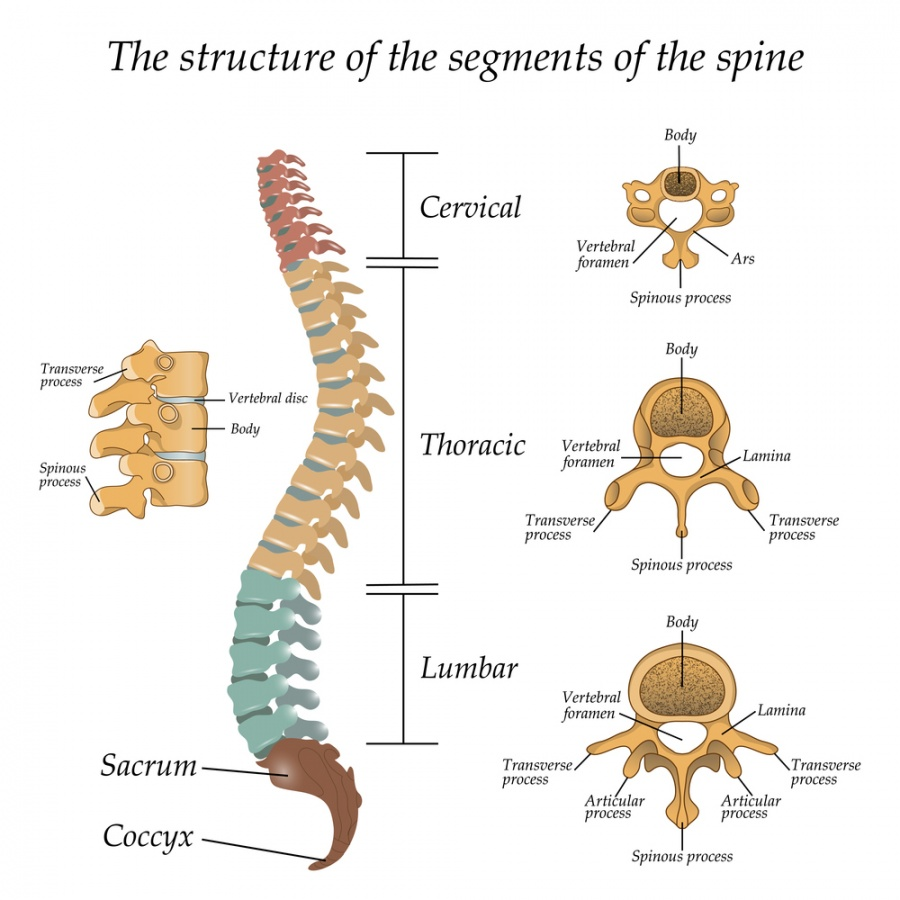
\includegraphics[width=10cm]{/home/thesis/images/SpineModel.jpeg}
    \caption{\label{fig:spineimage}Model of the human spine. The five vertebrae in green form the lumbar spine. They are referred to as \textit{L1} to \textit{L5} from top to bottom. Image source: \url{shutterstock.com}}
\end{SCfigure}

\section{Pathologies of the human spine}
\par{
    This document does not aim to provide an exhaustive list of all human spinal pathologies. 
    Two pathologies are interesting to discuss further as an introduction to this work since they occur in the data used in this project (see page \pageref{sec:datasets} for further details).
}
\begin{SCfigure}[][h!]
    \centering
    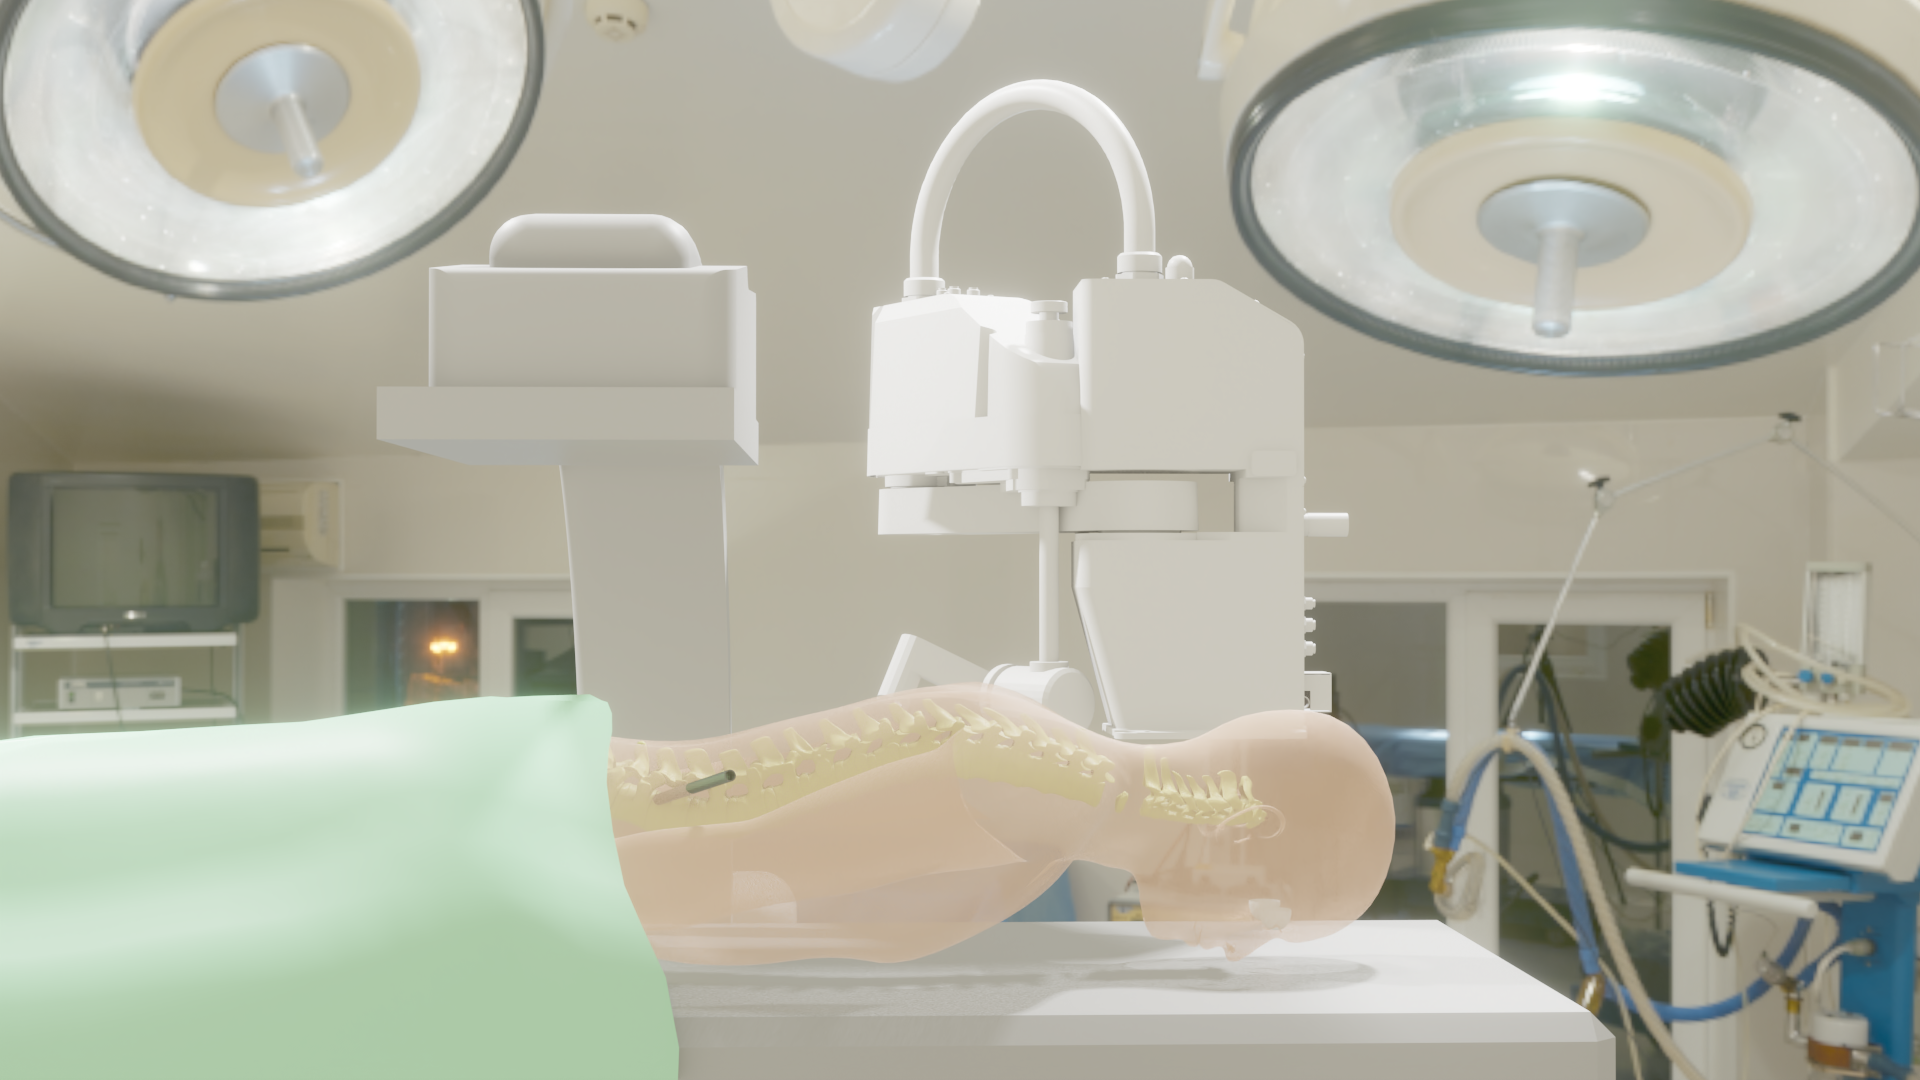
\includegraphics[width=10cm]{/home/thesis/images/REISS_illustration.png}
    \caption{Artist's impression of the start of the surgical treatment of a lumbar hernia. 
    This image shows the dilator through which the surgical instruments will be inserted to mill away the bulging disc material.
    This procedure requires repeated visualization of the instruments and the spine via X-ray images. \textit{This illustration is designed by Verhaert NP\&S}.\label{fig:REISS_procedure}}
\end{SCfigure}
\par{
    First, there is \textit{scoliosis}, which is a sideways curve of the spine.
    The severity of this condition can vary from relatively mild to severe. 
    In severe cases, scoliosis can affect the patient's movement and breathing.
}
\par{
    Second, there is the \textit{spinal hernia} or spinal disc herniation\footnote{Spinal disc herniation is sometimes referred to as a \textit{slipped disc}.}. 
    A spinal hernia is caused by damage to the \textit{annulus fibrosus}\footnote{The fibrocartilage ring around the softer gel-like centre of the intervertebral disc.}. 
    This damage can cause the intervertebral disc to bulge out. 
    This condition is painful due to the inflammation reaction, and in severe cases, the bulging material can irritate or cause impingement of the critical nerves along the spine.
    The nerve impingement can even lead to radiating pain to the limbs or even limb paralysis.
    In severe cases, a spinal hernia requires surgical treatment.
    This specialized procedure requires repeated medical imaging to allow the surgeon to accurately investigate the situation before the operation and assure correct positioning of the instruments during the intervention.
}
\par{
    In image \ref{fig:REISS_procedure}, the start of the surgical treatment procedure for a lumbar hernia is illustrated.
    One possible benefit of improved automatic interpretation of \acrshort{mri} and \acrshort{ct} scans is providing support for this procedure.
    This delicate procedure requires interpreting and registering information from both scan types (at different times), a demanding task for which automated support could be helpful.
    Image registration of the pre-operative \acrshort{mri} scan with the operation planning to the imaging of the situation on the operation table starts by segmentation of the affected vertebrae.
}

\section{Medical imaging of the human spine\label{sec:medical_imaging}}
\marginpar{
        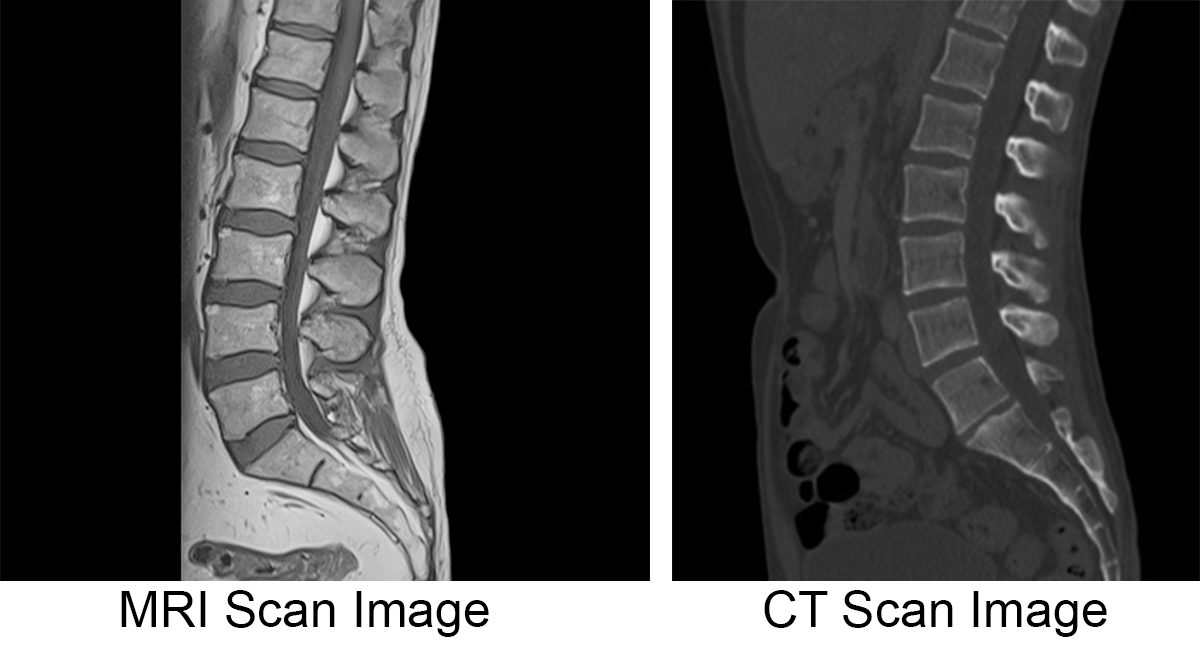
\includegraphics[width=5cm]{/home/thesis/images/MRI_CT_images.jpeg}
        \captionof{figure}{Illustration of \acrshort{ct} and \acrshort{mri} images of a human lumbar spine.}
        \label{fig:mri_ct}
    }
\par{
    For diagnosis and visualization of spinal pathology several medical imaging techniques are used: \acrfull{ct}, \acrfull{us} and \acrfull{mri}. 
    These techniques allow non-invasive visualization of the spine and discs in three dimensions.
    Slices from volumetric scans (\acrshort{mri} and \acrshort{ct}) are illustrated in \ref{fig:mri_ct}.
}

\subsection{CT scan}
\par{
    The \acrfull{ct}\footnote{Also known as CAT-scan, for Computed Axial Tomography or Computer-assisted Tomography.} is a non-invasive medical imaging procedure
    \footnote{\Gls{tomography} scans are primarily used for medical purposes. 
    It is also used in the industry for non-destructive inspection of components and assemblies.
    In geology, it is used to identify materials in a drill core quickly. In archaeology, it is used for the non-destructive investigation of artefacts. } 
    for diagnostic purposes. 
    A \acrlong{ct} procedure consists of the combination of an array of X-ray attenuation images taken with a rotating X-ray tube as illustrated in figure \ref{fig:CT_principle}. 
    These images can be combined with a \Gls{tomography} algorithm to reconstruct a volumetric representation of the radiographic density.
}
\par{
    Contrary to \acrfull{mri} imaging, this technique is suitable for patients with a pacemaker or insulin pump since there are no magnetic fields involved.
    The main disadvantage of \acrshort{ct} is the exposure to ionizing radiation\footnote{Radiation exposure increases the probability of cancer.} of the patient and the risk of exposure of the medical professional to the same radiation.
    The image quality increases with radiation dose, but so does the radiation exposure.
    Improving the reconstruction algorithms to obtain higher-resolution images while reducing radiation is an ongoing area of research. 
}
\marginpar{
        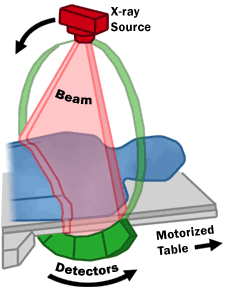
\includegraphics[width=5cm]{images/FDA_CT_Scan.png}
        \captionof{figure}{Conceptual illustration of the working of a \acrlong{ct} scan. Image from \url{www.fda.gov/radiation-emitting-products/medical-x-ray-imaging/computed-tomography-ct}}
        \label{fig:CT_principle}
    }

\subsection{MRI scan}
\par{
    The \acrfull{mri} scan is a medical imaging technique that is not based on ionizing radiation\footnote{Eventhough the alternative name \textit{nuclear} magnetic resonance (NMR) might confuse.}.
    \acrshort{mri} imaging will visualize the concentration of hydrogen\footnote{In theory, other atoms than hydrogen can be excited by adapting the excitation frequency.} atoms.
    The patient is positioned in a tunnel where a high constant magnetic field is applied. 
    A temporary oscillating signal is applied with the resonance frequency corresponding to hydrogen atoms is superposed on the static magnetic field.
    The hydrogen atoms will fall back to the equilibrium state, emitting radiofrequency (RF) signals, measured by receiving coils.
    \acrlong{mri} is particularly suitable for visualization of tissue with higher water content, such as tumours and infections, and to visualize fat.
}
\par{
    An \acrshort{mri} scan can be \textit{T1 weighted} or \textit{T2 weighted}. 
    A T1 weighted image is constructed based on the relaxation time of the magnetization is colinear with the direction of the static field
    while T2 weighted images are based on the magnetization perpendicular to the static field.
    While areas with higher water content, such as infected areas, will release a higher signal on a T2-weighted \acrshort{mri} scan, the same images will show a lower signal strength for T1-weighted scans.
}
\par{
    Contrary to \acrfull{ct} scans, the \acrlong{mri} procedure does not expose the patient of radiation. 
    Due to the high magnetic fields, the technology cannot be used for patients with pacemakers, cochlear implants or other metallic objects in the body.
    \acrshort{mri} allows to visualize soft tissue better than \acrshort{ct} images. An \acrshort{mri} image allows visualizing both the grey and white brain matter, while this is not possible with \acrshort{ct} images.
    Although both techniques produce images that resemble each other, none can replace the other one completely.
}


\chapter{Machine vision}

\Gls{machinevision} is the branch of \Gls{ai} focussed on image processing.
The machine vision task performed in this work is called instance \Gls{segmentation}.
In this chapter, I explain what this means. 
The task of segmentation is compared to other machine vision tasks.

This work investigates the used of \Gls{weaklysupervisedl} data for training an Instance segmentation model. 
The concept and benefits of \Gls{weaklysupervisedl} machine learning are explained.

\section{Machine vision tasks \label{sec:machinevisiontasks}}

\Gls{machinevision} is a broad discipline. 
Humans extract information from images almost subconsciously and we are often not aware of the different tasks we perform on images.
The objective of this section is to briefly define different machine vision tasks discussed further in this book. 
Several machine vision tasks consist of \textit{recognizing} objects, animals or humans in an image.
A model is build for a finite list of \textit{categories} that can be present in an image.
Depending on the question asked ad inference time, on can distinquish the following tasks.

\begin{description}
    \item[Image classification] is the task of determining what object category\footnote{or categories} is present in the image. Is there a cat in this image?
    \item[Object counting] is the task of counting how many instances of each category can be seen in the image. How many cats are there in this picture? 
    \item[Object detection] consists not only of identification of the object. Also the spatial position is requested. This is often requested in the form of a bounding box. Where is the cat in this picture, if a cat is present?
    \item[Semantic segmentation] requires that for each image pixel, a class is estimated. Pixels that do not belong to a specific class are called the \textit{background}.
    \item[Instance segmentation] requires not only that the semantic class is determined for each pixel, but also that two individuals of the same class\footnote{say, two cats.} are distinguished.   
\end{description}

The difference between these machine vision tasks is illustrated in figure \ref{fig:machinevisiontasks}. 

\begin{SCfigure}[][h!]
    \centering
    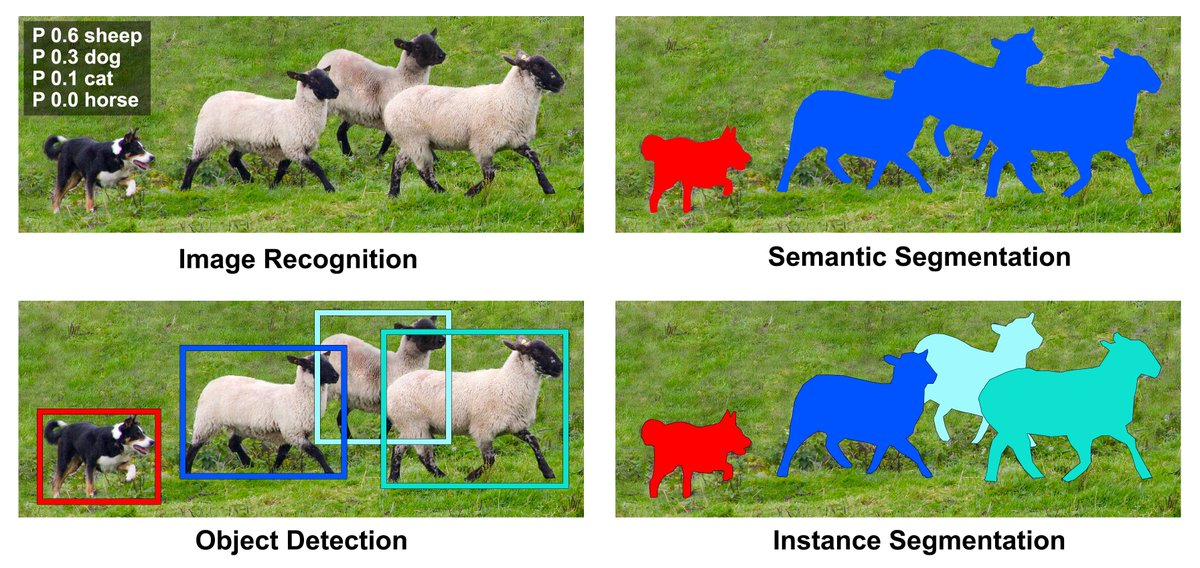
\includegraphics[width=10cm]{/home/thesis/images/Classification_vs_Segmentation.jpg}
    \caption{Illustration to compare different Machine vision tasks \cite{SemTorch76:online}. 
    Object detection means that the location of several objects is estimated by the model. This is indicated by the \textit{bounding boxes}.
    Segmentation of an image is the process of classifying each pixel in the correct class or assign it to the \textit{background} class.
    Semantic segmentation makes no difference between different instances of the same semantic class, instance segmentation does.
    \label{fig:machinevisiontasks}}
\end{SCfigure}

Other interesting applications of \gls{machinevision} include\footnote{This list is not exhaustive.}:
\begin{description}
    \item[Face recognition] is the identification of human faces. 
    \item[Image reconstruction] or \textit{inpainting} consists of recreating parts of a damaged image.
    \item[Image captioning] consists of the creation of full sentences describing the content of an image.    
\end{description}



\section{Supervision types}

To build a model to perform the tasks discussed in \ref{sec:machinevisiontasks}, this model needs to be trained.
This requires a set of \textit{labelled} images. 
This means that a collection of images needs to be provided where an expert in the intended task has provided correct information the model can \textit{learn} from.
Depending on the model objective, other types of labelling are required.
Figure \ref{fig:ImageLabelTypes} illustrates several types of image supervision : 
Point supervision, squiggle, bounding box and full mask.
The generation of these labels is very expensive and time-consuming.
Especially \gls{deepl} models are known to be very data-hungry. 
These models have determined unprecedented performance, provided sufficient data has been provided.

\begin{SCfigure}[][htb]
    \centering
    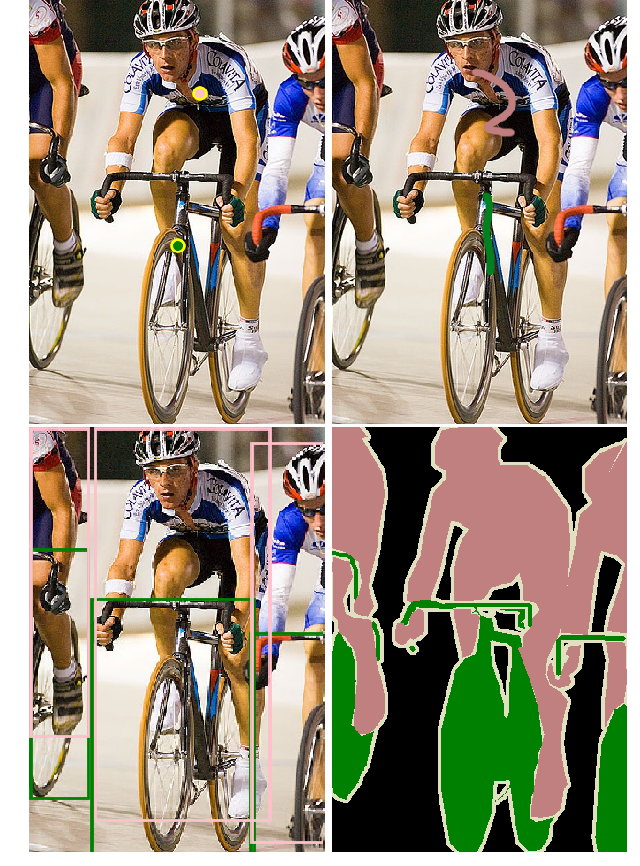
\includegraphics[width=10cm]{/home/thesis/images/McEver.png}
    \caption{Four different annotation types \cite{McEver2020}: 
    On the top left the picture is point level annotated. The points are inflated for visibility.
    On the top right, squiggle annotation is used.
    The bottom left shows bounding box supervion.
    While the bottom right image is fully annotated.
    An image level label would indicate that there are multiple instances of \textit{person} and \textit{bike} in the image.
    \label{fig:ImageLabelTypes}}
\end{SCfigure}

Given the high labelling cost, several researchers have investigated ways to train computer vision models with cheaper labels.
This branch of research is known as \Gls{weaklysupervisedl}.
The objective is to construct a strong model based on \textit{cheap} (incomplete, noisy or imprecise) labels. 
This is sometimes described as \textit{indirect supervision}.
Numerous creative approaches have been conceived. 
It is impossible to give an exhaustive list of approaches. 
In what follows, I will mainly focus on the approaches I chose to investigate myself, but I will also try to give some hints of the remarkable creativity found in the field.
Since the provided annotations in \Gls{weaklysupervisedl} are not full labels, these are sometimes described as \textit{hints} instead\footnote{
    This is based on the insightfull talk at \url{
        https://youtu.be/4EjYxVVCAaE
    }. For example, the destinction between labels and hints.
}.
The basic concept of \Gls{weaklysupervisedl} is that there are two sources of information to draw from: The hints and the prior knowledge about the problem (Priors).
These \textit{Priors} can be any form of prior knowledge about the object to be segmented\footnote{or any other machine vision task.}.
Priors can be the object size, shape or location, the number of instances, the similarity across images or the similarity with exernal images.

Wether an annotation is considered a \textit{weak label} or a \textit{strong label} depends more on the modellers intend than on the annotation itself. 
Basically, when one aims to construct a model to infer output labels with a higher informative value than the original annotations, these \textit{labels} become \textit{hints}.
Making a model to predict bounding boxes from a dataset annotated with bounding boxes means considering these as \textit{strong labels}. 
If one uses the same dataset to construct a model that predicts pixel-wise masks, you use the labels as \textit{weak labels} or \textit{hints}.

For a segmentation task, weak labels can be:
\begin{description}
    \item[Image level labels]: When only  
\end{description}

\todo[inline]{Motivation of weakly supervised learning --> Difference in annotation time and cost from Bearman and Laradji Covid}
\chapter{Previous work}

This project sits at the intersection of two areas of research. 
First there is the application of \Gls{ai} in medical applications, specifically for segmentation problems.
Then, there is the active area of research of \Gls{weaklysupervisedl} machine learning.

\section{Artificial intelligence for medical applications}

\todo[inline]{Start with short overview of other AI problems (~5 lines)}

\Gls{ai} has proven to be a valuable contribution to medical practice to reduce the burden of repetitive tasks on the medical caregiver.

\todo[inline]{elaborate: ppg to blood pressure - slaapapnue}

\section{Segmentation problems for medical applications}

\todo[inline]{General introduction of U-Net and other medical approaches}

For segmentation tasks, the U-net \cite{Ronneberger2015} is widely used. 
This architecture can be represented by a characteristic U-shape, as the name indicates.
It consists of 

\begin{SCfigure}[][htb]
    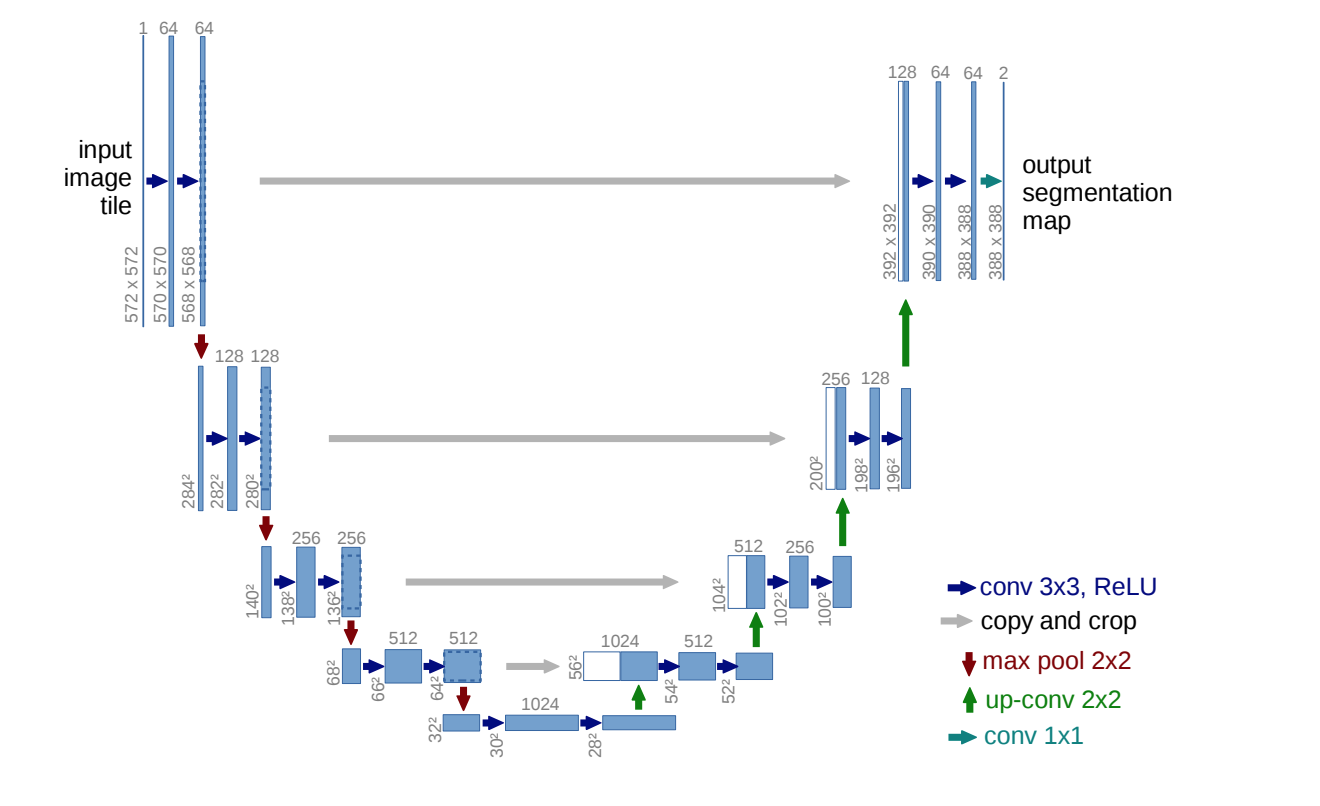
\includegraphics[width=10cm]{/home/thesis/images/UNet_Ronneberger.png}
    \caption{U-Net architecture, as illustrated in \cite{Ronneberger2015}. 
    Each blue box represents a multi-channel feature-map. 
    The number of channels is indicated above the box, the $x \times y$ dimensions are indicated at the bottom left.
    The gray arrows indicate the feature maps in the contracting path are copied and concatenated to the feature maps of the expanding path.}
    \label{fig:unet}
\end{SCfigure}

\todo[inline]{General introduction of U-Net and other medical approaches}

\subsection{Segmentation of the human spine}

\todo[inline]{other authors, approaches --> priors used, metrics used}

\section{Weakly supervised segmentation}

\subsection{General approaches}

\todo[inline]{How is this problem generally solved: PCAMS, WISE, ...}

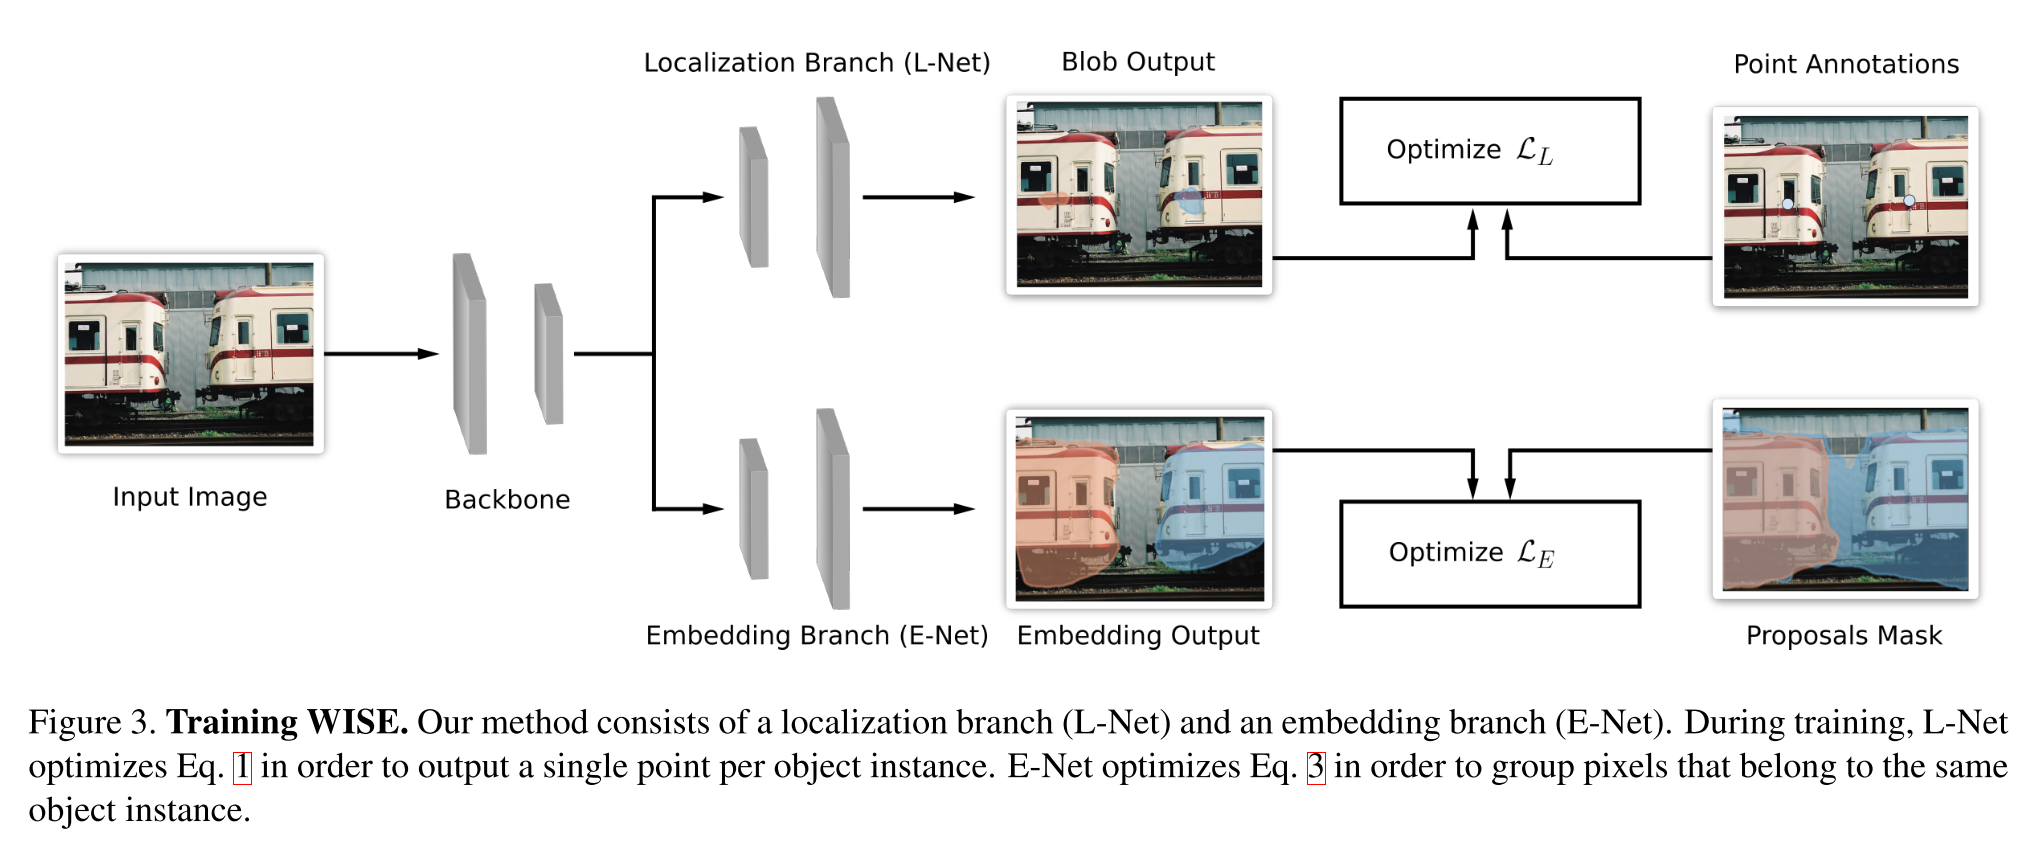
\includegraphics[width=10cm]{/home/thesis/images/Laradji_architecture.png}
\captionof{figure}{Architecture of the U-net based segmentation}
\label{fig:laradji}

\subsection{Weakly supervised segmentation for Medical applications}

Laradji COVID 19


\newgeometry{total={210mm,297mm},left=30mm,right=30mm,bindingoffset=5mm, top=25mm,bottom=25mm} 
\begin{partwithabstract}{Modelling methods \& Analysis}
  \par{
    This part of the document details the used datasets and the modelling and evaluation methodology.
    First, and overview is provided of the 5 datasets used in this work.
    Statistics regarding the patient's age and gender are documented for the sets for which this metadata is available. 
  }
  \par{
    Second, the data preparation steps are explained, before describing the modelling approach, the network architectures and the model loss functions.
  }
    
\end{partwithabstract}
\restoregeometry

\chapter{Datasets}

This thesis is based on 5 different already existing datasets.
This chapter discusses these datasets based on different criteria:

\begin{description}
    \item[source:] reference of the owner of the dataset and brief description of the original purpose of the dataset. Importantly, this part also discusses the source of the annotation.
    \item[Patient sample:] statistics of the patients of whom medical images were collected such as age, gender and possible spine pathologies.
    \item[Technical information:] discusses the imaging technology, the image resolution and the spatial dimensions of the image. 
\end{description}

\section{Global overview of the different dataset}

\todo[inline]{Overview of the datasets gathered. MRI / CT, number of images, type of annotation + WHO performed the annotation? Was it a medical docter or one of the researchers.}



bla

\begin{SCtable}[\sidecaptionrelwidth][h]
 
    \begin{tabular}{ l l l l l} 
     \hline
     \hline
     Name & reference & imaging & Quantity & Annotation \\
          &           & technology & [images] & \\
     \hline 
    UWSpine & \cite{Glocker}  & \acrshort{ct} & 125 & point  \\ 
    xVertSeg & \cite{Ibragimov2014, Korez2015} & \acrshort{ct} & 15 & full \\
    UniSiegen  & \cite{Zukic2014} & \acrshort{mri} & 17 & full \\
    PLoS & \cite{Chu2015} & \acrshort{mri} & 23 & semantic \\
    MyoSegmenTUM & \cite{Burian2019} & \acrshort{mri} &  54 & full \\
     \hline
     \hline
    \end{tabular}
    \caption{List of dataset references. For more details on the data quantity, please consult chapter \ref{seg:datasetcomparison}. 
    Notably the fact that some images were taken from the same patient is important. This means the dataset is grouped. 
    The agreement with prof. T. Vrtovec regarding the xVertSeg dataset can be found in appendix \ref{seg:datasetagreement}.}

\end{SCtable}

\begin{SCtable}[\sidecaptionrelwidth][h]
 
    \begin{tabular}{ l l l l} 
     \hline
     \hline
     Name & X & Y & Z \\
     \hline 
    UWSpine & Left-right & Anteroposterior & Craniocaudal \\
    xVertSeg & Left-right & Anteroposterior & Craniocaudal \\
    UniSiegen  &  Anteroposterior & Craniocaudal & Left-right \\
    PLoS & Left-right & Anteroposterior & Craniocaudal$^\dagger$ \\
    MyoSegmenTUM &  Anteroposterior & Craniocaudal & Left-right \\
     \hline
     \hline
    \end{tabular}
    \caption{List of dataset references. For more details on the data quantity, please consult chapter \ref{seg:datasetcomparison}. 
    Notably the fact that some images were taken from the same patient is important. This means the dataset is grouped. 
    The agreement with prof. T. Vrtovec regarding the xVertSeg dataset can be found in appendix \ref{seg:datasetagreement}.
    $^\dagger$ The Craniocaudal axis in the PLoS dataset is inverted.}

\end{SCtable}

\section{Comparison of the different datasets\label{seg:datasetcomparison}}


\subsection{xVertSeg\label{sec:xVertSeg}}



The xVertSeg \cite{Ibragimov2012, xxx} was kindly made available by prof. T. Vrtovec (University of Ljubljana, Faculty of Electrical Engineering, Slovenia), see appendix \ref{seg:datasetagreement} for the agreement.
This dataset contains 25 \acrfull{ct} scans of the lumbar spine, of which 15 \acrshort{ct} scans are fully labeled.
Given the provided data, I can assume these 15 scans were collected from 15 different patients.

For each of these 15 scans, full instance segmenation masks for all 5 lumbar vertebrae are provided. The delineation was performed by a skilled professional.

Additionally, for each vertebra a fracture class and fracture grade is provided. 
Apart from vertebrae classified as \textit{normal}, the dataset contains \textit{mild}, \textit{moderate} and \textit{severe} cases of vertebrae fracture types \textit{wedge}, \textit{crush} and \textit{biconcavity}.
\marginpar{
        % This file was created by tikzplotlib v0.9.8.
\begin{tikzpicture}

\definecolor{color0}{rgb}{0.917647058823529,0.917647058823529,0.949019607843137}
\definecolor{color1}{rgb}{0.298039215686275,0.447058823529412,0.690196078431373}
\definecolor{color2}{rgb}{0.768627450980392,0.305882352941176,0.32156862745098}

\begin{axis}[
axis background/.style={fill=color0},
axis line style={white},
height=5cm,
tick align=outside,
tick pos=left,
width=5cm,
x grid style={white},
xlabel={Gender},
xmajorgrids,
xmin=0.5, xmax=2.5,
xtick style={color=white!15!black},
xtick={1,2},
xticklabels={F (8),M (7)},
y grid style={white},
ylabel={Patient age [y]},
ymajorgrids,
ymin=0, ymax=100,
ytick style={color=white!15!black}
]
\addplot [color1, opacity=1]
table {%
0.925 66
1.075 66
1.075 79.25
0.925 79.25
0.925 66
};
\addplot [color1, opacity=1]
table {%
1 66
1 60
};
\addplot [color1, opacity=1]
table {%
1 79.25
1 90
};
\addplot [black, opacity=1]
table {%
0.9625 60
1.0375 60
};
\addplot [black, opacity=1]
table {%
0.9625 90
1.0375 90
};
\addplot [black, mark=o, mark size=3, mark options={solid,fill opacity=0}, only marks]
table {%
1 40
};
\addplot [color1, opacity=1]
table {%
1.925 73.5
2.075 73.5
2.075 78.5
1.925 78.5
1.925 73.5
};
\addplot [color1, opacity=1]
table {%
2 73.5
2 73
};
\addplot [color1, opacity=1]
table {%
2 78.5
2 82
};
\addplot [black, opacity=1]
table {%
1.9625 73
2.0375 73
};
\addplot [black, opacity=1]
table {%
1.9625 82
2.0375 82
};
\addplot [black, mark=o, mark size=3, mark options={solid,fill opacity=0}, only marks]
table {%
2 56
};
\addplot [color2, opacity=1]
table {%
0.925 72.5
1.075 72.5
};
\addplot [color2, opacity=1]
table {%
1.925 77
2.075 77
};
\end{axis}

\end{tikzpicture}

        \captionof{figure}{xVertSeg patients age distribution}
        \label{fig:xVertSeg_Age}
    }

\subsubsection{Original Objective of the Dataset}

The objective of the \textit{xVertSeg challenge}\footnote{see \url{http://lit.fe.uni-lj.si/xVertSeg/database.php}} (2015) was organized by the University of Ljubljana.
Based on the 15 provided scans with corresponding masks, the participans were required to construct a model to make predictions on the test set of 10 unlabelled scans.

The challenge consisted of two tasks:
\begin{enumerate}
    \item Segmentation of the lumbar vertebrae. For each scan in the test set, the segmentation masks of the lumbar vertebrae were requested.
    \item Fracture classification on the segmented vertebrae, consisting of morphological grade and fracture classification.
\end{enumerate}

\subsubsection{Patient statistics}

The patients in the xVertSeg dataset train set consist of 8 females and 7 males.
The age of these patients is slightly higher than for the other datasets.
The average patient in this dataset is 71 years old.
A box plot of the age distribution between genders is shown in figure \ref{fig:xVertSeg_Age}. 

\begin{SCtable}[\sidecaptionrelwidth][h]
    \centering
        \begin{tabular}{lrrrrrr}
\toprule
{} &  L1 &  L2 &  L3 &  L4 &  L5 &  Total \\
\midrule
biconcave &   6 &   7 &   8 &   4 &   2 &     27 \\
normal    &   5 &   6 &   4 &   4 &   7 &     26 \\
wedge     &   3 &   2 &   2 &   3 &   2 &     12 \\
crush     &   1 &   0 &   1 &   4 &   4 &     10 \\
\bottomrule
\end{tabular}

        \caption{Every patient in the xVertSeg dataset suffers from at least one spine pathology.
        Most of these pathologies are identified as \textit{mild}.
        This table counts the spine pathologies and normal vertebrae observed over all 15 patients in the xVertSeg dataset.}   
\end{SCtable}

\subsubsection{Technical information}

The xVertSeg dataset contains 15 \acrshort{ct} annotated scans. 
This dataset is very interesting due to the high quality and high resolution of the images.
On figure \ref{fig:xVertSeg_image002}, two slices of the same patient (002) are represented.
The slices show the complete, uncropped sections of the torso and abdominal region of the patient. 
There is no \acrshort{roi} cropping.

\begin{SCfigure}[][htb]
    \centering
    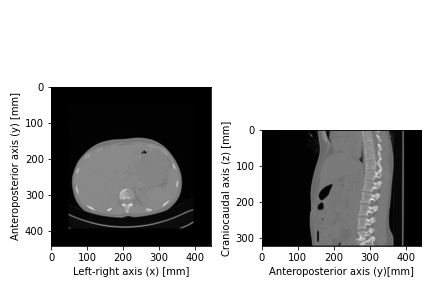
\includegraphics[width=.95\textwidth]{automated_graphs/xVertSeg_image002.png}
    \caption{xVertSeg scan \textit{image002}. \label{fig:xVertSeg_image002}}
\end{SCfigure}

The distribution of the scan dimensions is shown in figure \ref{fig:AllDataset_dims}. This also illustrates the \textit{xVertSeg} dataset consists of large, high resolution images.
Mind that during pre-processing the scans are resampled on a $1mm \times 1mm \times 1mm$ grid.


\subsection{UniSiegen dataset\label{sec:DataUSiegen}}

This dataset is made available in 2014 by the University of Siegen, Germany.
Dr D. Zukic \cite{Zukic2014} constructed it as part of his PhD project.

\marginpar{
        % This file was created by tikzplotlib v0.9.8.
\begin{tikzpicture}

\definecolor{color0}{rgb}{0.917647058823529,0.917647058823529,0.949019607843137}
\definecolor{color1}{rgb}{0.298039215686275,0.447058823529412,0.690196078431373}
\definecolor{color2}{rgb}{0.768627450980392,0.305882352941176,0.32156862745098}

\begin{axis}[
axis background/.style={fill=color0},
axis line style={white},
height=5cm,
tick align=outside,
tick pos=left,
width=5cm,
x grid style={white},
xlabel={Gender},
xmajorgrids,
xmin=0.5, xmax=2.5,
xtick style={color=white!15!black},
xtick={1,2},
xticklabels={F(11),M(6)},
y grid style={white},
ylabel={Patient age [y]},
ymajorgrids,
ymin=0, ymax=100,
ytick style={color=white!15!black}
]
\addplot [color1, opacity=1]
table {%
0.925 21.5
1.075 21.5
1.075 38.5
0.925 38.5
0.925 21.5
};
\addplot [color1, opacity=1]
table {%
1 21.5
1 21
};
\addplot [color1, opacity=1]
table {%
1 38.5
1 55
};
\addplot [black, opacity=1]
table {%
0.9625 21
1.0375 21
};
\addplot [black, opacity=1]
table {%
0.9625 55
1.0375 55
};
\addplot [black, mark=o, mark size=3, mark options={solid,fill opacity=0}, only marks]
table {%
1 74
1 69
};
\addplot [color1, opacity=1]
table {%
1.925 33
2.075 33
2.075 69.5
1.925 69.5
1.925 33
};
\addplot [color1, opacity=1]
table {%
2 33
2 27
};
\addplot [color1, opacity=1]
table {%
2 69.5
2 72
};
\addplot [black, opacity=1]
table {%
1.9625 27
2.0375 27
};
\addplot [black, opacity=1]
table {%
1.9625 72
2.0375 72
};
\addplot [color2, opacity=1]
table {%
0.925 22
1.075 22
};
\addplot [color2, opacity=1]
table {%
1.925 58
2.075 58
};
\end{axis}

\end{tikzpicture}

        \captionof{figure}{USiegen patients age distribution}
        \label{fig:USiegen_Age}
    }

This dataset contains 26 \acrshort{mri} scans of 17 different patients\footnote{This is not clearly stated, but can be inferred from the metadata.}. 
The fact that scans of the same patient are correlated will be taken into account in the train, validation and test split.
For more details on this split, see section \ref{sec:trainValTestSplit} on page \pageref{sec:trainValTestSplit}.

\subsubsection{Original Objective of the Dataset}

This dataset was collected from several hospitals (Sarajevo, Marburg, Brisbane, Schwabach, Bad Wildungen \& Prague). The MRI scanner settings were varied between the scans (T1, T2, TIRM).
The PhD project objective was to build a segmentation model to automate the segmentation of the lumbar vertebrae in the \acrshort{mri} scans to facilitate the diagnosis of several spine pathologies 
such as scoliosis, spondylolisthesis \footnote{Spondylolisthesis is the displacement of one spinal vertebra compared to another.} and vertebral fractures.
The final model developed by dr. D. Zukic consisted of a Viola-Jones detector for detection and vertebral body size approximation.
The average Dice score compared to the manual reference was reported to be 79.3\%.

\subsubsection{Patient statistics}

In \cite{Zukic2014}, it is not entirely made clear which scans are taken from the same patient.
It is made clear, however that the 26 scans were not obtained from 26 patients.
The information was inferred from the naming of the scans and the provided gender en age information\footnote{
    Wrongfully assuming two scans come from the same patient does not cause data leakage.
}.

Figure \ref{fig:USiegen_Age} illustrates that the USiegen dataset contains almost double the number of female patients compared to male patients.
These patients are relatively young compared to the patients in the \textit{xVertSeg} dataset.

Only three of the patients in this dataset were categorized as having no spinal pathologies.

\subsubsection{Technical information}

Several \acrlong{mri} techniques were used to obtain the dataset: T1, T2 \& TIRM.
I do not take into account this factor in the model development or the dataset split.

The volumes in the USiegen dataset are strongly cropped. 
Both in the anteroposterior and the craniocaudal direction, the volumes are on average 370 mm.
In the left-right direction, however, the volumes have been cropped severely. The volumes are, on average, only 68 mm wide.
The images have been cropped to only include the \acrshort{roi}.
Along this left-right dimension, the voxel spacing is large. 

\begin{SCfigure}[][htb]
    \centering
    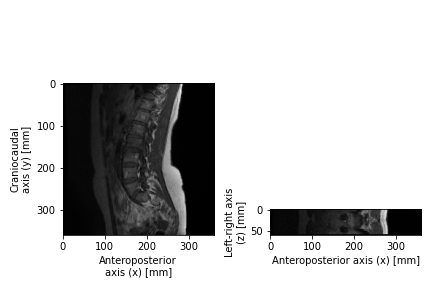
\includegraphics[width=.95\textwidth]{automated_graphs/USiegen_Aka3.png}
    \caption{USiegen dataset scan \textit{Aka3}. \label{fig:USiegen_Aka3}. It is immediately clear the USiegen volumes are cropped differently than the xVertSeg volumes.
    In the craniocaudal direction, both sacrum and coccyx are visible. Along the left-righ axis, the volumes have been cropped severely.}
\end{SCfigure}

The original scans in the \textit{USiegen} dataset were cropped in the \textit{left-right} direction. 
Although the scan resolution is relatively high in the Sagittal planes, the slice spacing along the left-right axis is coarser (see figure \ref{fig:AllDataset_dims}).  
\subsection{PLoS Dataset}

The \textit{PLoS} dataset was compiled for \cite{Chu2015} in 2015 by dr. C. Chu, University of Bern, Bern, Switzerland and made publically available \footnote{See : \url{ http://doi.org/10.5281/zenodo.22304 }} .
It consists of 23 T2-weighted spine \acrshort{mri} scans. 
Contrary to other datasets, the segmenation labels in this dataset do not provide information to destinguish the individual vertebrae from each other.

\subsubsection{Original Objective of the Dataset}

In \cite{Chu2015} the development of a random forest regression approach for spine vertebrae segmenation and classificiation is described.
The results of several random forest regressors and classifiers is unified with a voting mechanism.
This approach obtains a mean Dice metric score of 88.7\%.

\subsubsection{Patient statistics}

Due to the anomimization process, the \textit{PLoS} dataset does not contain patient information.
This means that it is not possible to produce any statistics regarding patient age or gender.

\subsubsection{Technical information}

As is indicated in figure \ref{fig:AllDataset_dims}, and in figure \ref{fig:PLoS_img02}, the PLoS image volumes are cropped in the left-right direction.
The volumes are consistently $381mm \times 381 mm \times 78 mm$, where the shortest dimension is in the left-right direction.

\begin{SCfigure}[][htb]
    \centering
    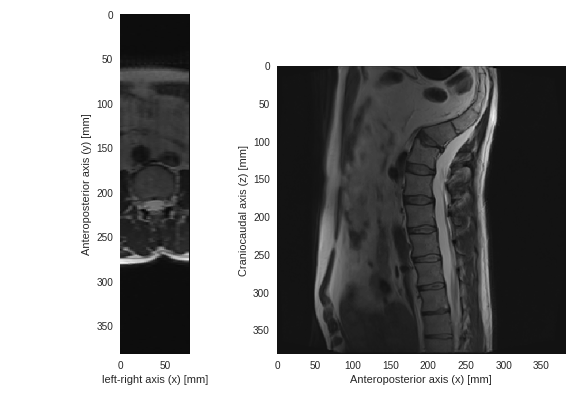
\includegraphics[width=.95\textwidth]{automated_graphs/PLoS_img02.png}
    \caption{
        PLoS dataset scan \textit{img02}. \label{fig:PLoS_img02}. The craniocaudal direction is cropped in a way comparable to the volumes in the USiegen dataset, but, the direction of this axis is inverted.
        The left-right axis is cropped similar to the USiegen data volumes.
    }
\end{SCfigure}
\subsection{MyoSegmenTUM datset}

This dataset is made available by S. Schläger from the Technische Universität München via the \acrfull{osf} \footnote{see \url{ https://osf.io/3j54b/?view_only=f5089274d4a449cda2fef1d2df0ecc56 }}.
It was constructed for the MyoSegmenTUM project \cite{Burian2019}.
It consists of 54 collections of \acrshort{mri} scans of the spine.
In this work, only the T2 weighted \acrlong{mri} scans are used.
The dataset also contains volumes with enhanced fat tissue response. Since the objective of this work is related to bone tissue rather than fat tissue, these volumes were not used.
Neither was the segmentation masks for the different dorsal muscles, which are also present in this dataset.

\subsubsection{Original Objective of the Dataset}

The MyoSegmenTUM Spine dataset is compiled as a reference dataset for developing segmentation algorithms of the lumbar spine vertebral bodies and muscle groups.
Information about this project can be found in \cite{Burian2019}.

\subsubsection{Patient statistics}

In figure \ref{fig:OSF_ageboxplot}, the age distribution of the patients in the MyoSegmenTUM dataset is shown.
There are more women (39) included in this dataset than men (15).
The male patients in this dataset are, on average, clearly younger than the female patients.

\marginpar{
        % This file was created by tikzplotlib v0.9.8.
\begin{tikzpicture}

\definecolor{color0}{rgb}{0.917647058823529,0.917647058823529,0.949019607843137}
\definecolor{color1}{rgb}{0.298039215686275,0.447058823529412,0.690196078431373}
\definecolor{color2}{rgb}{0.768627450980392,0.305882352941176,0.32156862745098}

\begin{axis}[
axis background/.style={fill=color0},
axis line style={white},
height=5cm,
tick align=outside,
tick pos=left,
width=5cm,
x grid style={white},
xlabel={Gender},
xmajorgrids,
xmin=0.5, xmax=2.5,
xtick style={color=white!15!black},
xtick={1,2},
xticklabels={F(39),M(15)},
y grid style={white},
ylabel={Patient age (y)},
ymajorgrids,
ymin=18.1666324435318, ymax=80.5007186858316,
ytick style={color=white!15!black}
]
\addplot [color1, opacity=1]
table {%
0.925 32.5
1.075 32.5
1.075 62.7652292950034
0.925 62.7652292950034
0.925 32.5
};
\addplot [color1, opacity=1]
table {%
1 32.5
1 21
};
\addplot [color1, opacity=1]
table {%
1 62.7652292950034
1 77.6673511293635
};
\addplot [black, opacity=1]
table {%
0.9625 21
1.0375 21
};
\addplot [black, opacity=1]
table {%
0.9625 77.6673511293635
1.0375 77.6673511293635
};
\addplot [color1, opacity=1]
table {%
1.925 27
2.075 27
2.075 33
1.925 33
1.925 27
};
\addplot [color1, opacity=1]
table {%
2 27
2 23
};
\addplot [color1, opacity=1]
table {%
2 33
2 41
};
\addplot [black, opacity=1]
table {%
1.9625 23
2.0375 23
};
\addplot [black, opacity=1]
table {%
1.9625 41
2.0375 41
};
\addplot [color2, opacity=1]
table {%
0.925 58.2888432580424
1.075 58.2888432580424
};
\addplot [color2, opacity=1]
table {%
1.925 31
2.075 31
};
\end{axis}

\end{tikzpicture}

        \captionof{figure}{Distribution of patient age in the dataset from the MyoSegmenTUM project.}
        \label{fig:OSF_ageboxplot}
    }


\subsubsection{Technical information}

As shown in figure \ref{fig:OSF_02}, coupes from the second volume of the MyoSegmenTUM dataset are shown.
As is also indicated in figure \ref{fig:AllDataset_dims}, the dimensions of the MyoSegmenTUM volumes is consistent $220 mm \times 220 mm \times 80 mm$, where the shortest dimension is the cropped left-right axis.
There are only three volumes that deviate slightly from this.

\begin{SCfigure}[][htb]
    \centering
    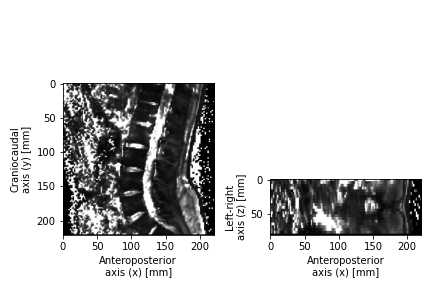
\includegraphics[width=.95\textwidth]{automated_graphs/OSF_02.png}
    \caption{MyoSegmenTUM dataset scan \textit{02}. 
    The volumes are cropped in the left-right direction. 
    \label{fig:OSF_02}}
\end{SCfigure}

\textbf{Remark:} For three volumes (nr 33, 53 and 54) for which the dimension of the image volume and the label mask do not correspond. 
It is not clear how these masks should be used. 
These volumes were discarded, bringing the final number of volumes used from the MyoSegmenTUM dataset to 51.
\subsection{UWSpine dataset}
 
This dataset is made available by the Department of Radiology of the University of Washington\footnote{Creative Commons Attribution-NonCommercial-NoDerivatives 4.0 International License, dataset available at \url{
      https://biomedia.doc.ic.ac.uk/data/spine/  
    }}.
It has been constructed by dr. Glocker and team \cite{Glocker2012,Glocker2013} (Microsoft research) in 2012.
For each scan, manual annotations of vertebrae centroids are provided.
This dataset contains 242 \acrshort{ct} scans of 150 different patients.
This dataset does not contain full mask labels, only centroid point annotations.
To investigate the relative performance of a weakly supervised model compared to the performance of a fully supervised model, both will be trained on the same dataset\footnote{The modelling concept is further discussed in chapter \ref{sec:model_concept}.}.
Furthermore, the evaluation of the models is based on the full annotations.
Thus, the UWSpine dataset will not be used for model training.
It will only be used for visual evaluation of the model on a completely new dataset\footnote{The UWSpine dataset is \textit{completely} new in the sense that no samples from this dataset (this \textit{population}, so to speak) are present in the train or validation set.
For the \textit{normal} test set, other samples from the same datasets where present in the train and validation sets.}.


\subsubsection{Original Objective of the Dataset}

In \cite{Glocker2012,Glocker2013} the development of a model based on regression forests and a \acrfull{hmm} for vertebra localisation without needing strong assumptions on what part of the spine is visible.

\subsubsection{Patient statistics}


Figure \ref{fig:UW_ageboxplot} illustrated that the patients in the \textit{UWSpine} dataset are relatively varied in age.
Of most patients in the dataset, multiple scan images are available.
The highest number of scans taken from a single patient is 5.

\subsubsection{Technical information}

Only point annotations are available for the \textit{UWSpine} dataset. 
This means this dataset can only be used for weakly supervised model training.

The scans in the \textit{UWSpine} dataset are strongly cropped around the spine, both in the left-right direction and the anteroposterior direction.

\begin{SCfigure}[][htb]
    \centering
    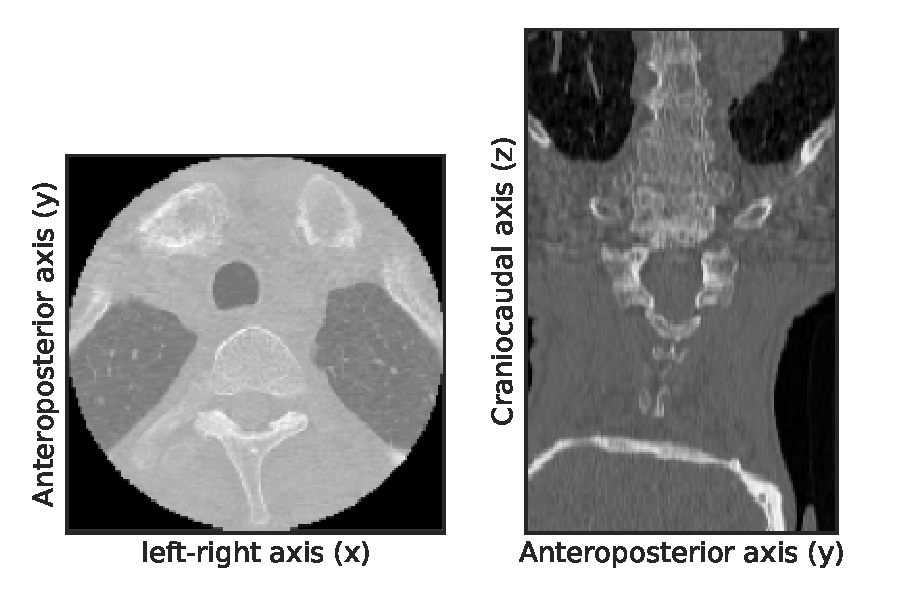
\includegraphics[width=.95\textwidth]{automated_graphs/UW_4564688.pdf}
    \caption{University of Washington dataset, scan \textit{4564688}. \label{fig:UW_4564688}}
\end{SCfigure}

\marginpar{
        % This file was created by tikzplotlib v0.9.8.
\begin{tikzpicture}

\definecolor{color0}{rgb}{0.917647058823529,0.917647058823529,0.949019607843137}
\definecolor{color1}{rgb}{0.298039215686275,0.447058823529412,0.690196078431373}
\definecolor{color2}{rgb}{0.768627450980392,0.305882352941176,0.32156862745098}

\begin{axis}[
axis background/.style={fill=color0},
axis line style={white},
tick align=outside,
tick pos=left,
x grid style={white},
xlabel={Gender},
xmajorgrids,
xmin=0.5, xmax=2.5,
xtick style={color=white!15!black},
xtick={1,2},
xticklabels={Female (54 patients),Male (71 patients)},
y grid style={white},
ylabel={Patient age (y)},
ymajorgrids,
ymin=11.05, ymax=97.95,
ytick style={color=white!15!black}
]
\addplot [color1, opacity=1]
table {%
0.925 42.75
1.075 42.75
1.075 64.75
0.925 64.75
0.925 42.75
};
\addplot [color1, opacity=1]
table {%
1 42.75
1 15
};
\addplot [color1, opacity=1]
table {%
1 64.75
1 94
};
\addplot [black, opacity=1]
table {%
0.9625 15
1.0375 15
};
\addplot [black, opacity=1]
table {%
0.9625 94
1.0375 94
};
\addplot [color1, opacity=1]
table {%
1.925 41.5
2.075 41.5
2.075 65.5
1.925 65.5
1.925 41.5
};
\addplot [color1, opacity=1]
table {%
2 41.5
2 15
};
\addplot [color1, opacity=1]
table {%
2 65.5
2 90
};
\addplot [black, opacity=1]
table {%
1.9625 15
2.0375 15
};
\addplot [black, opacity=1]
table {%
1.9625 90
2.0375 90
};
\addplot [color2, opacity=1]
table {%
0.925 54
1.075 54
};
\addplot [color2, opacity=1]
table {%
1.925 54
2.075 54
};
\end{axis}

\draw ({$(current bounding box.south west)!0.5!(current bounding box.south east)$}|-{$(current bounding box.south west)!0.98!(current bounding box.north west)$}) node[
  scale=0.6,
  anchor=north,
  text=white!15!black,
  rotate=0.0,
  align=center
]{OSF dataset
age distribution};
\end{tikzpicture}

        \captionof{figure}{Distribution of patient age in the dataset from Washington University.}
        \label{fig:UW_ageboxplot}
    }


% Data preparation part
\chapter{Data preprocessing}

The available data volumes have to be preprocessed before being used in the neural network classifier.
The preprocessing steps consist of resampling, slicing, contrast enhancement and cropping.  

There is not one obvious way to combine the different datasets and available labels in one project.
The chosen approach in this work is discussed below.
First, the conversion of the full class labels to point labels is discussed. 
Secondly, the split of the datafiles in a train set, a validation set and a test set is discussed.

\section{Image preprocessing}

A (medical) image\footnote{In this work, I use \textit{image} to refer both to 2-dimensional and 3-dimensional images.} consists of a combination of data - the pixel
\footnote{A \textit{pixel} (picture-element) is the smallest component of a digital bitmap image. 
It is defined by a position vector and carries $c$ values. Where $c$ is the number of channels of the image. 
Sometimes, a pixel of a 3-dimensional digital image is called a \textit{voxel} (volume element).} 
values - and metadata.

For a medical image, there are two types of metadata:
\begin{description}
    \item [Describing the patient \& medical data:] patient identification, pathologies, date of scan, date of birth, gender, weight, height,\dots
    \item [Technical meta-data:] The size (number of pixels per dimension), pixel spacing (distance between pixels along a dimension), orientation vector, image modality \& other information regarding the image acquisition.
\end{description}

For a discussion of the data used in this work, chapter \ref{sec:datasets} can be consulted. 

\subsection{Resampling and slicing\label{sec:resampling}}

In figure \ref{fig:AllDataset_dims}, the differences regarding the dimension and resolution for the different volumes in the combined dataset are illustrated. 
It is necessary to uniformize the data input to the network. 
This requires uniformization of the image spacing vector in all directions\footnote{A typical \acrshort{cnn} is not scale-invariant.}. 
I chose to resample on a $1mm\times 1mm \times 1mm$ isotropic grid. 
If necessary, images are rotated to uniformize the orientation vectors. 
Every image is now a 3-dimensional array\footnote{Both \acrshort{ct} and \acrshort{mri} images have only one channel.} with the same sequence of dimensions and the same spacing along these dimensions.
The chosen uniform dimension sequence is:
\begin{enumerate} 
    \item Craniocaudal axis; perpendicular to the transverse plane.
    \item Anteroposterior axis; perpendicular to the coronal (frontal) plane.
    \item Left-right axis; perpendicular to the sagittal plane.
\end{enumerate}
The inputs for the 2D models are obtained by \textit{slicing} the volume along with one of the dimensions.
This means that from each scan volume, three different sets of two-dimensional slices can be generated, depending on the slicing axis\footnote{The slicing axis is the axis perpendicular to which ones slices the volume}.

When resampling the image itself, linear interpolation is used. 
To resample the classification masks on a new grid, the \textit{nearest neighbour} method is used\footnote{
    SimpleITK \cite{sitk} provides useful tools to perform these operations.
    } 
since factorial data must not be interpolated. 

\subsection{Contrast enhancement}
To two-dimensional images obtained from slicing, the volumes are preprocessed with the \acrfull{clahe} algorithm. 
The difference with ordinary histogram equalization is that the \acrshort{clahe} method calculates different histograms for different sections of the image.
This technique allows improving the local contrast in each region of an image.
When an image contains regions that are significantly lighter or darker than the rest of the image (as is the case for both \acrshort{ct} and \acrshort{mri} images), the AHE methods perform better than histogram equalization based on the complete image.

\begin{SCfigure}[][htb]
    \centering
    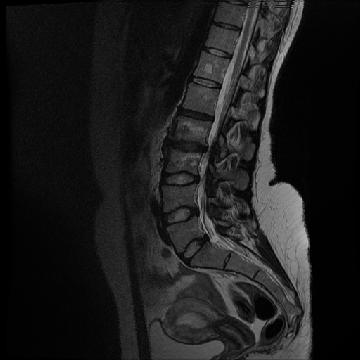
\includegraphics[width=.32\textwidth]{images/orig_usieg8_s22.jpg}
    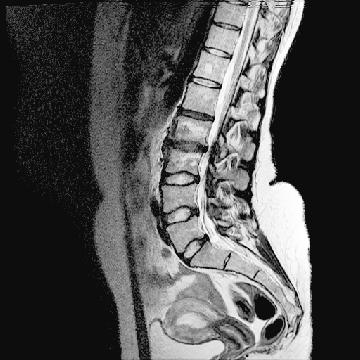
\includegraphics[width=.32\textwidth]{images/hist_usieg8_s22.jpg}
    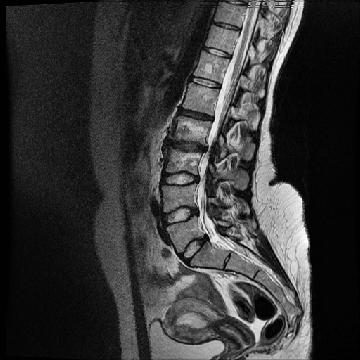
\includegraphics[width=.32\textwidth]{images/clahe_usieg8_s22.jpg}
    \caption{Image: 22$^{th}$ sagittal slice of the 8$^{th}$ image of the USiegen dataset. 
    From left to right, the original image, the image after ordinary histrogram contrast enhancement and the result after \acrshort{clahe}.
    The images show that \acrshort{clahe} avoids increasing the noise in the larger dark areas while resulting in a more balanced image than the ordinary histogram method.
    }
\end{SCfigure}

\acrfull{clahe} is an improvement on adaptive histogram equalization.
Limiting the contrast amplification avoids that noise is amplified in (near) constant regions of the image.
The parameters of this operation were adjusted manually.
Based on trial and error iterations, where the quality of the contrast improvement was estimated with the human eye based on visualizations from all datasets,
the following parameters were chosen:
\begin{description}
    \item[Number of grey bins:] 256 (maximum possible when working with 8-bit encoded images).
    \item[Kernel size:] 50. This parameter defines the extent of the \textit{local} region used by the algorithm.
    \item[clip limit:] $9.10^{-3}$. This parameter suppresses noise in the darkest regions (which contain the least information).
\end{description}

\newpage
\section{Train, validation and test split considerations\label{sec:trainValTestSplit}}

To allow evaluation of the models produced, a test set is split from the development set.
The objective is to evaluate how well a model generalizes to new data\footnote{
    New data is to be interpreted here as a new sample from \textit{the same population} as the development sample.
    Unfortunately, I cannot claim that the different datasets I collected indeed form a perfect representation of the population of medical images of the lumbar spine.}. 
To provide an honest estimate of the out-of-sample performance, the test dataset should represent the investigated population and (hidden) correlations with elements of the development sample should be avoided.

This is done\footnote{
    To accomplish this, I used the function \texttt{GroupedStratifiedSplit} at \url{https://github.com/scikit-learn/scikit-learn/pull/18649/}. 
    This class is not yet part of the official \texttt{sci-kit learn} library release (at the time of writing) but functions well for this application.} taking into account the following:
\begin{description}
    \item[Stratified data:] The combination of data from different sources is stratified. Every source is considered a subpopulation. The data split is made such that the proportion of scans originating from each data source in every split is proportional to their occurrence in the total population.
    \item[Grouped data:] The scans of the same patient can be assumed to be correlated to each other. These scans should not be spread over different splits. The data is split at patient level.
\end{description}

For each datasource, the intended split is $\frac{4}{6}$ for train set, $\frac{1}{6}$ for cross validation set and $\frac{1}{6}$ for test set.
This distribution is not perfect but acceptable, as is indicated by the values in table \ref{tab:summary_split}.

\begin{SCtable}[\sidecaptionrelwidth][h]
 
    \begin{tabular}{lrrr}
\toprule
split &  test &  train &  xval \\
source       &       &        &       \\
\midrule
MyoSegmenTUM &     9 &     33 &     9 \\
PLoS         &     4 &     14 &     4 \\
USiegen      &     2 &     14 &     1 \\
xVertSeg     &     2 &     10 &     3 \\
\bottomrule
\end{tabular}

    \caption{Number of volumes by datasource and by split.\label{tab:summary_split}}
  
  \end{SCtable}

  \begin{SCtable}[\sidecaptionrelwidth][h]
 
    \begin{tabular}{ll|lll|l}
    \toprule
    split        &            & test & train & xval & total \\
    source       & dimension  &      &       &      &       \\ \midrule
    MyoSegmenTUM & Transverse & 1989 & 7293  & 1989 & 11271 \\
                 & Frontal    & 1989 & 7293  & 1989 & 11271 \\
                 & Sagittal   & 720  & 2650  & 725  & 4095  \\
    PLoS         & Transverse & 1528 & 5348  & 1528 & 8404  \\
    USiegen      & Transverse & 733  & 5063  & 501  & 6297  \\
                 & Frontal    & 681  & 4276  & 1080 & 6037  \\
                 & Sagittal   & 145  & 1089  & 180  & 1414  \\
    xVertSeg     & Transverse & 759  & 2652  & 785  & 4196  \\
                 & Frontal    & 812  & 4163  & 1290 & 6265  \\
                 & Sagittal   & 812  & 4163  & 1290 & 6265  \\ \midrule
    total        & Transvers  & 5009 & 20356 & 4803 & 30168 \\
                 & Frontal    & 3482 & 15732 & 4359 & 23573 \\
                 & Sagittal   & 1677 & 7902  & 2195 & 11774 \\ \bottomrule
    \end{tabular}
    \caption{Number of slices by datasource and by split.\label{tab:summary_split_slices}}
  
  \end{SCtable}

The result of this operation is detailed in appendix \ref{sec:appendix_split} on page \pageref{sec:appendix_split}.

\section{Cropping\label{sec:cropping}}
The networks used require input images of size $352 p \times 352 p$, corresponding to $352 mm \times 352 mm$.
The image slices have different dimensions.
The incoming images are cropped or padded, depending on whether the image dimension is smaller or larger than the crop window.


When the image is cropped, one of 5 crops is selected, see figure \ref{fig:crop}:
\begin{description}
    \item[crop 0:] Crop from the top left corner of the image.
    \item[crop 1:] Crop from the top right corner of the image.
    \item[crop 2:] Crop from the bottom left corner of the image.
    \item[crop 3:] Crop from the bottom right corner of the image.
    \item[crop 4:] Center crop of the image.  
\end{description}

Not all slices are sufficiently large to produce 5 different crops. This is illustrated in figure \ref{fig:smallcrop}. In this case, one of the slice dimensions must be padded (symmetrically) to obtain an image of the desired dimensions.

When a slice is fetched from the train set, a random crop is selected from these 5.
This adds an extra level of variance to the training data. This avoids, for example, that the network learns that the spine is always at the same location in the images.

For the slices sourced from the cross-validation and train set, however, reproducibility is essential.
For each slice, the crop number is fixed.
This way, the cross-validation metric, evaluated to avoid overfitting is always calculated on the same images.

When reconstructing the volumes, in the second step of the model concept (see chapter \ref{sec:model_concept}), 
all different crops are evaluated in the model, and the responses for these crops are joined by averaging the model responses in the overlap regions.

\begin{SCfigure}[][htb]
    \centering
    \begin{minipage}{.99\textwidth}
        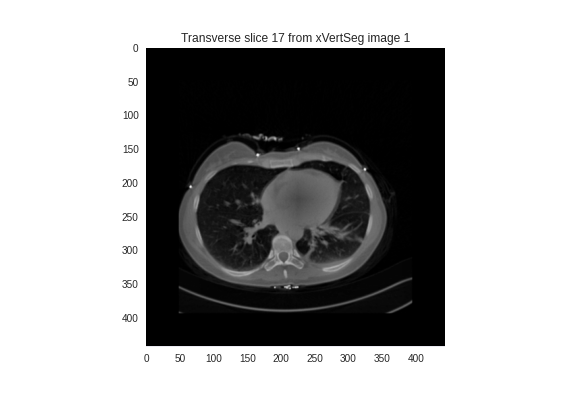
\includegraphics[width=.99\textwidth]{images/slice017.png}
    \end{minipage} 
    \begin{minipage}{0.99\textwidth}
        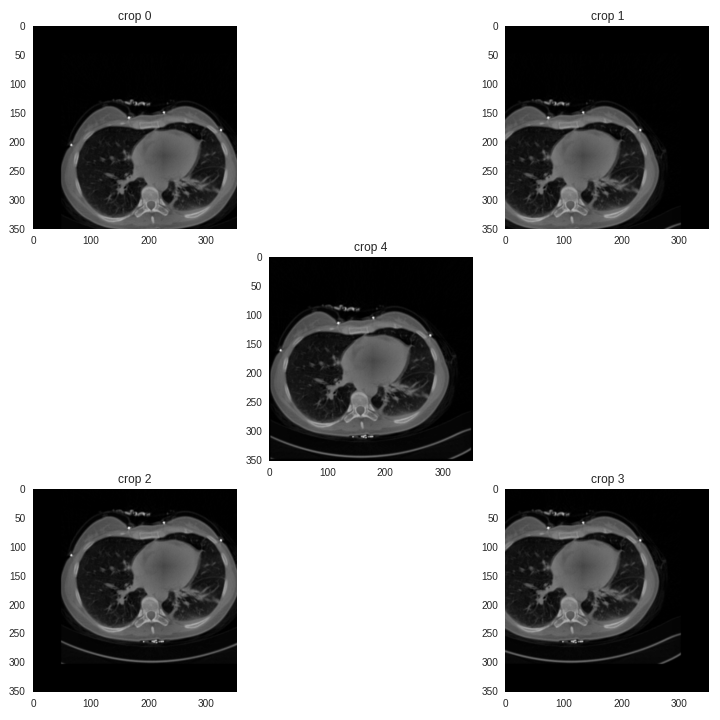
\includegraphics[width=.99\textwidth]{images/cropping_slice017.png}
    \end{minipage}
    \caption{
        Illustration of image cropping where the image is larger than the crop window dimensions. The original size of the image is $443 \times 443$, and the crop window used has dimensions $352 \times 352$.
        Crop 0 to 4 are 5 different images but have a considerable overlap. \label{fig:crop}
        }
    
\end{SCfigure}

\begin{SCfigure}[][htb]
    \centering
    \begin{minipage}{.99\textwidth}
        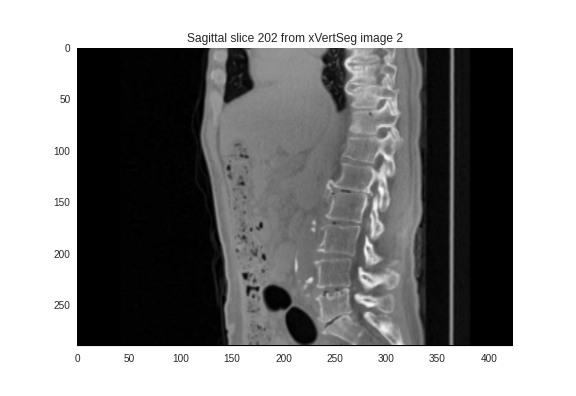
\includegraphics[width=.99\textwidth]{images/slice202.png}
    \end{minipage} 
    \begin{minipage}{0.99\textwidth}
        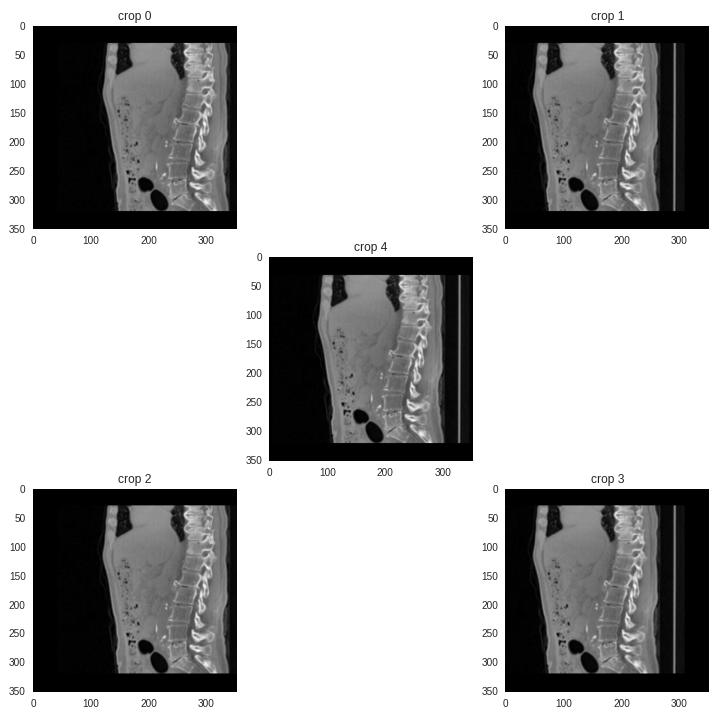
\includegraphics[width=.99\textwidth]{images/cropping_slice202.png}
    \end{minipage}
    \caption{
        Illustration of image cropping where the image is larger than the crop window dimensions.
        The original size of the image is $291 \times 424$, and the crop window used has dimensions $352 \times 352$.
        Crop 0 to 4 are not all different images. Since the image height is lower than the crop window height, this dimension is padded, not cropped.
        This results in crop 0 being equal to crop 2 and crop 1 being equal to crop 3. \label{fig:smallcrop}
        }
    
\end{SCfigure}

\chapter{Modelling methods \& evaluation protocols}\thispagestyle{empty}
\par{
    This chapter introduces the high-level model concept of this work.
    This consists of producing pseudo masks from three weakly supervised models trained on different sets of slices obtained from the same volume.
    Next, the construction, training and evaluation of these weakly supervised models are covered in more detail.
    Attention is given to the model loss function, including two loss components that add to the consistency loss framework\cite{Laradji2021}.
    Finally, the model evaluation metrics are described.
    These metrics will be used to compare the result of the \Gls{weaklysupervisedl} model with the result of a model trained on fully supervised labels.
    Both models will be trained on the same test scans, and the model performances will be evaluated on the same test scans.
}
\section{Modelling concept}

\subsection{Model type}

The main model concept is the use of a 2D \acrfull{cnn} to provide 3D segmentation masks, trained on point annotated data.
Out-of-the-box pre-trained 2D networks are available, with weights pre-trained on enormous public datasets\footnote{\label{footnote:Imagenet}For example, weights trained on the ImageNet dataset. 
This dataset consists of \todo[inline]{xxx} images of xxx categories.}.
An alternative approach would be to use 3D networks. This is a logic choice for volumetric data, with the obvious advantage that the 3D convolution layers naturally take into account the structure of the data.
One could argue that using 2D networks deprives the network of important \textit{context} information in the direction perpendicular to the slice it is analysing (I try to meet this issue in section \ref{section:twoDplus} on page \pageref{section:twoDplus}). 

There are also advantages to choosing 2D networks over 3D networks:
\begin{enumerate}
    \item Since the number of parameters (weights) to train scales exponentially with the kernel dimension, the number of parameters to train is considerably higher for a 3D \acrshort{cnn} compared to a corresponding 2D \acrshort{cnn}.
    \item The academic community has been investigating 2D \acrlong{cnn}s for a longer time. The networks can be initialized with weights pretrained on very large and diverse datasets (see remark \ref{footnote:Imagenet} on ImageNet). 
    These datasets indeed do not contain the specific classes, nor the specific datatype investigated in this project. 
    The different convolution layers have proven however to extract useful general features that allow the network to distinguish a very wide range of categories. 
    These features have proven to be sufficiently general to be applicable to new machine vision applications. This practice is called transfer learning \todo{references}.
    \item Although consecutive slices are obviously strongly correlated, one has more data\footnote{There are more slices than volume segments in 1 image volume.} to train the networks. Certainly when considered in proportion to the number of weights to be trained.
\end{enumerate}

\subsection{Model training approach}

An approach used often in weakly supervised learning is the generation of \textit{ersatz} full mask labels.
In this project, I intended to use this approach too.

A scan volume can be sliced along 3 different axis: the transverse axis, the coronal axis and the sagittal axis. 
This means that 3 different models can be trained with the available point annotated data. 
Each of these 3 networks will have different context elements to segment the sliced images on.
The resulting segmentation volumes\footnote{The segmentation results of a stack of 2D slices can be combined to form a 3D segmentation volume.} of these three networks can then be combined to obtain a final segmentation volume.
This final segmentation mask, which should be as least as good as the best of the 3 individual model results, can then be used as \textit{ersatz} masks to train a final \textit{fully supervised} network. 

\begin{SCfigure}[][htb]
    \centering
    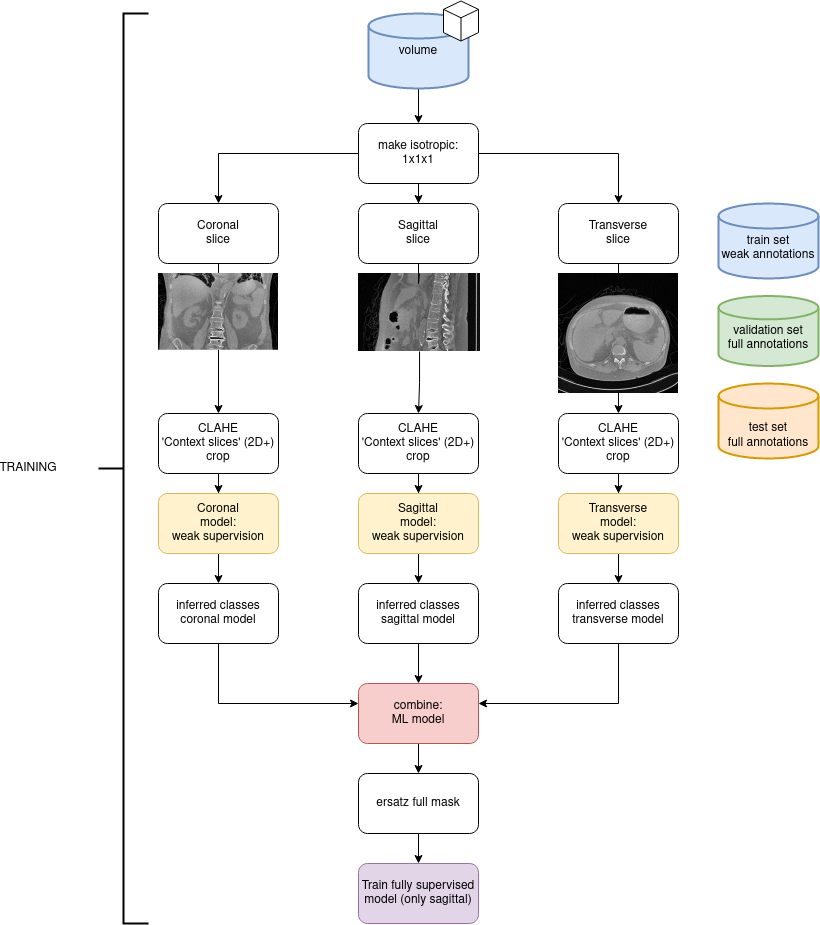
\includegraphics[width=.85\textwidth]{/home/thesis/images/Training_concept.png}
    \caption{\label{fig:model_training_concept}Illustration of the model training approach. 
    This is based on the conbination of 3 different models based on different volume slices.}
\end{SCfigure}

When the segmentation masks of a new, unknown volume need to be inferred, only this final model needs to be evaluated.

\begin{SCfigure}[][htb]
    \centering
    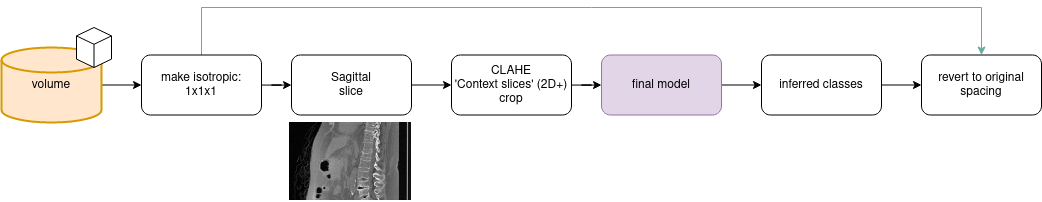
\includegraphics[width=.95\textwidth]{/home/thesis/images/Inference_concept.png}
    \caption{Inference step. Only one model needs to be evaluated in this step, the model that is trianed in the final step of the training procedure illustrated in figure \ref{fig:model_training_concept}.}
\end{SCfigure}
\FloatBarrier
\section{Hyperparameter overview}

Building the different models for the procedure illustrated in figure \ref{fig:model_training_concept} requires to make a number of choices.
In this section, these components are introduced.

\subsection{Network types\label{sec:network_types}}

Three different \acrlong{cnn} architectures were tested for this project:
\begin{description}
    \item[the VGG16 network: ] classic, added some upscore layers.
    \item[The RESNET50 network:] skip connections
    \item[The U-Net network: ] good performance for some biological problems
\end{description}

All of these networks function based on the \textit{encoder - decoder} principle.
\todo{add more insights on the principle}

\begin{SCfigure}[][htb]
    \centering
    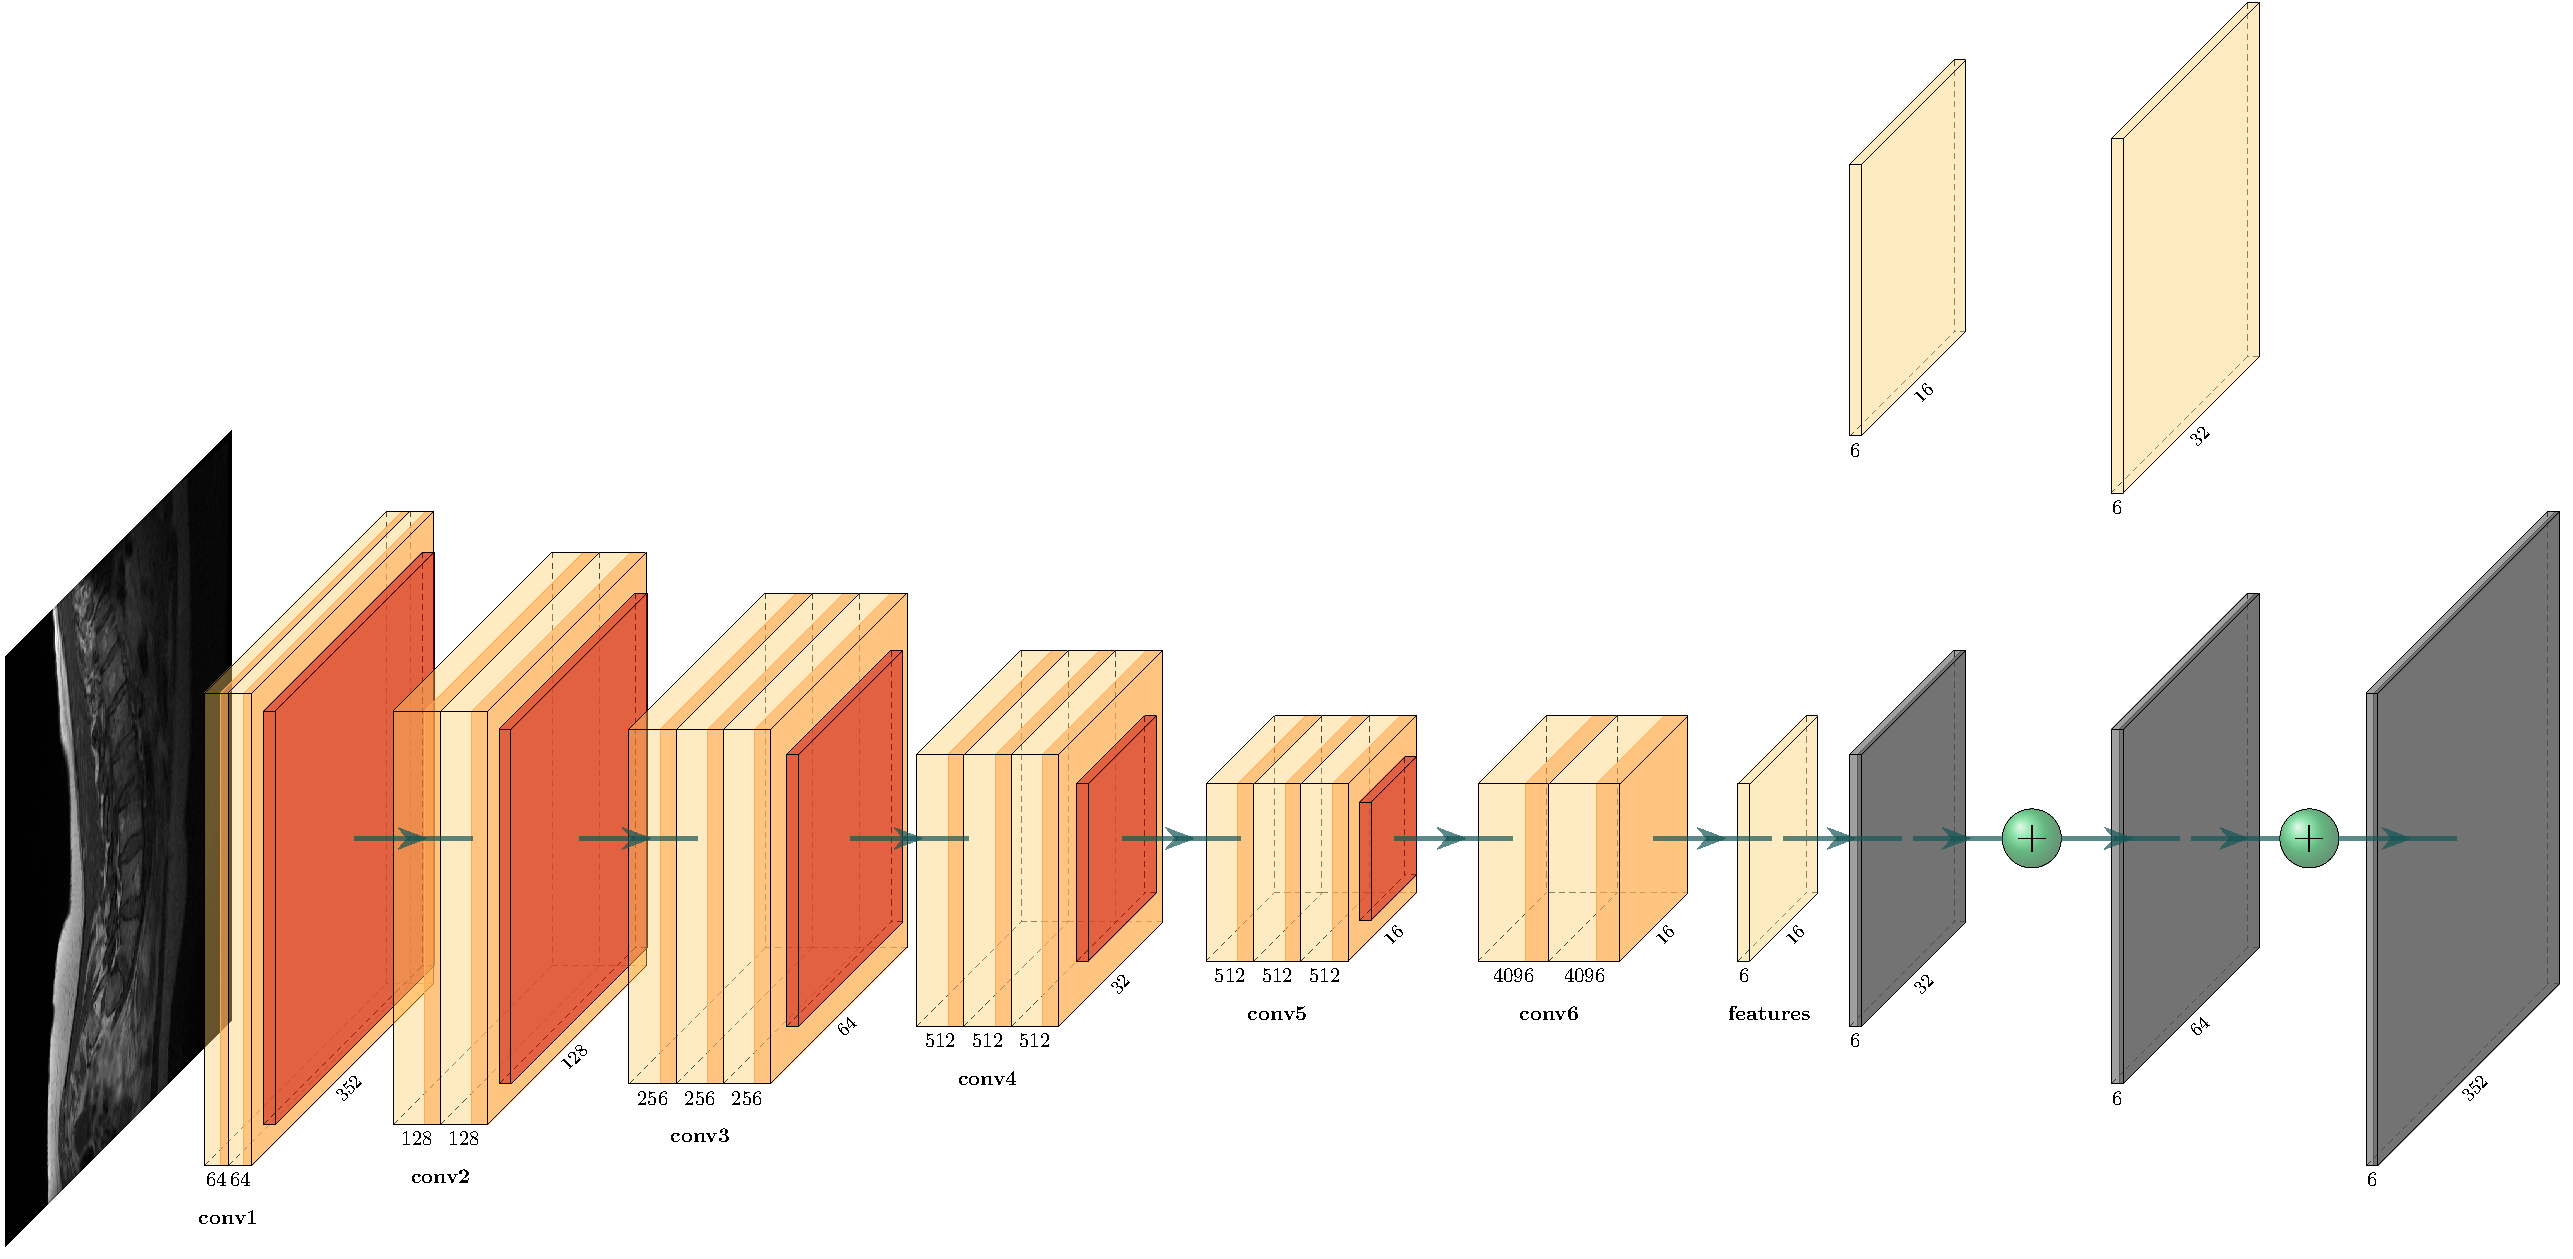
\includegraphics[width=.95\textwidth]{vgg16_upscore.pdf}
    \caption{VGG16 based network}
\end{SCfigure}

\begin{SCfigure}[][htb]
    \centering
    \includegraphics[width=.95\textwidth]{unet.pdf}
    \caption{Unet based network}
\end{SCfigure}

\subsection{2D+ approach and \textit{context slices}\label{section:twoDplus}}

As discussed in section \ref{sec:network_types}, all used networks have a 3 channel\footnote{The networks were originally designed for \textit{RGB}-images with a red, a green and a blue channel.}, 
352$\times$352 pixel input. 
The input images for the network only have 1 channel component. 
The other two channels were used to pass \textit{context} information to the network in the form of the neighboring slices of the slice under investigation.
This combines an essentially 2D approach with a third dimensional element in the form of the extra information of the parallel slices. Thus, this is called the $2D+$ approach.


The hyperparameter to be set $k$ is the index offset for the context slices.
When evaluating slice with index $n$ the slices with indices $\left[n-k; n+k\right]$ are passed as context slices
\footnote{For the edge cases ($n<k$ or $n+k>$ image dimension) when these slices do not exist, slice $n$ is passed as context slice.}.


Several values for $k$ are tested. When $k=0$, no extra slices are taken. The same slice is just entered in all 3 network channels. When $k=1$, the indices directly next to the investigated slices are taken.
Due to the isotropic resampling (see section \ref{sec:resampling}), these slices are physically at 1 mm distance of the center slice. When $k=5$, the slices at $5 mm$ distance from the center slice are used.

\section{Loss functions\label{sec:LossFunctions}}
\par{
    Construction of a machine learning model requires evaluating the model, comparing the result of this evaluation with the desired output and taking steps to make the observed output resemble the desired output better.
    In other words, to train a model, the optimizer will minimize the loss function.
    To use the gradient descent algorithm, this loss function needs to be differentiable.
}
\par{
    Several loss components will be discussed below, both unsupervised and supervised loss functions.
    A supervised loss function component considers the difference between the network prediction and a known (weak) label.
    An unsupervised loss function component considers characteristics of the network output itself. No labels are used in calculating an unsupervised loss component.
    The desirable characteristics that are enforced by the unsupervised loss functions can be part of the \textit{priors}, the knowledge on the problem one has beforehand
    \footnote{To be able to work with weaker, less informative labels, one needs to enter more prior knowledge into the problem}. 
}
In order to make the notation in this section clearer, table \ref{tab:loss_notations} list the notations used in the loss function components.
\begin{SCtable}[\sidecaptionrelwidth][h]
 
    \begin{tabular}{ l l } 
     \hline
     \hline
     Symbol & meaning \\
     \hline 
    $n$                 & Number of problem classes \\
    $X_i$               & Slice $i$ and corresponding context slices   \\ 
    $\vec{p}$           & A pixel position in slice $i$ \\
    $\mathcal{K}$       & Set of outcome classes: $\mathcal{K} = [0, 1, \dots, n-1]$ \\
    $\mathcal{Y}_i$     & set of labels for slice $i$, $\mathcal{Y}_i(\vec{p}) \in \mathcal{K}$  \\
    $\mathcal{I}_i$     & set of pixel positions for which a label is available \\
    $f_\theta(X_i)=z_i$ & model output (logits) for $X_i$ with weights $\theta$. $\vec{z_i(\vec{p})}\in \mathbb{R}^n$ \\
    $\sigma(z_i(\vec{p}))$   & softmax result for $\vec{z_i(\vec{p})}$ ($\in \mathbb{R}^n$ and $\forall k\in \mathcal{K} 0\leq\sigma_k\leq1$) \\
    $w_k$ & A weigth that can be attributed to class $k \in \mathcal{K}$ \\
     \hline
     \hline
    \end{tabular}
    \caption{List of symbols used in the loss functions\label{tab:loss_notations}}

\end{SCtable}
\par{
    In this project, $n=6$ for the coronal and sagittal slice models and $n=2$ for the transverse slice models. 
    Label $\mathcal{Y}_i(\vec{p})=0$ indicates the background class and the lubar vertebrae $L_m$ are indicated with $\mathcal{Y}_i(\vec{p})=m$ ($m\in[1,2,3,4,5]$).
    In the fully supervised case, $\mathcal{I}_i$ spans the complete slice $i$. In the weakly supervised case, there are only a handful of positions $\vec{p}$ for which a label exists.
}
The softmax function $\sigma$ is related to the sigmoid function $\mathbf{S}$. It is defined as:

\begin{eqnarray}
    \sigma_k(z) &=& \frac{\exp(z_k)}{\sum_{m\in\mathcal{K}} \exp(z_m)} \\
    \mathbf{S}(x) &=& \left[ 1+ exp(-x) \right]^{-1} \\ &=& \frac{exp(x)}{exp(x) + 1} 
\end{eqnarray}

The final training loss is given by:
\begin{equation}
    \mathcal{L} = \mathcal{L}_P + \mathcal{L}_E + \mathcal{L}_C + \mathcal{L}_S
\end{equation}
The different loss components are detailed below.

\subsection{Supervised loss functions}

\subsubsection{cross entropy loss\label{sec:crossentropy} \& Point loss}
To compare the network output with the labels, first, the (weighted) cross entropy loss is used\footnote{The weight is optional. One can decide $\forall i\in\mathcal{K}: w_i=1$}.

\begin{equation}
\mathcal{L}_P(X_i) = -\sum_{\vec{p} \in \mathcal{I}_i} w_{\mathcal{Y}_i(\vec{p})}.\log\left[\sigma_{\mathcal{Y}_i(\vec{p})}\left(\vec{z_i(\vec{p})}\right)\right]
\label{eq:LP}
\end{equation}

This loss term is minimized when the network output $z_i(\vec{p})[k]$ with $k=\mathcal{Y}_i(\vec{p})$ the class label for $\vec{p}$ is maximal while the other logits for this position are minimal.
In the fully supervised case, this loss function is called the cross entropy loss. 
When training a model with point supervision, this is only one of multiple loss components. 
In the case of point supervised data, $\mathcal{I}_i$ only consists of a handful of points.
This loss component is in this case called the point loss component $\mathcal{L}_P$.

\subsubsection{Prior extend loss}
The second supervised loss function used is the \textit{prior extend} loss.
This loss function describes the prior knowledge that the dimensions of a vertebra are limited. 
Based on \cite{Alam2014}, the maximal extent of a human lumbar vertebrae was set to be $r=110mm$.
This means that a point label $\mathcal{Y}_i(\vec{p})=m: m\in[1,2,3,4,5]$ indicating that $\vec{p}$ is a point in vertebra $L_m$, also means that all points outside of a cicle with radius $r$ cannot be points of $L_m$.
\marginpar{
        % This file was created by tikzplotlib v0.9.8.
\begin{tikzpicture}

\begin{axis}[
height=5cm,
tick align=outside,
width=5cm,
x grid style={white!69.0196078431373!black},
xmin=-0.5, xmax=349.5,
xtick pos=both,
xtick style={color=black},
y dir=reverse,
y grid style={white!69.0196078431373!black},
ymin=-0.5, ymax=349.5,
ytick pos=left,
ytick style={color=black}
]
\addplot graphics [includegraphics cmd=\pgfimage,xmin=-0.5, xmax=349.5, ymin=349.5, ymax=-0.5] {images/prior_extend-000.png};
\addplot [draw=black, fill=black, mark=*, only marks, scatter]
table{%
x  y
120 80
100 35
};
\end{axis}

\end{tikzpicture}

        \captionof{figure}{Illustration of the prior extend mask for annotation points at [120, 80] and [100, 34]. In the grey area, $\mathbf{m} = 0$.}
        \label{fig:prior_extent}
    }
First, $n-1$ (in this case 5) distance masks are created\footnote{1 label is background, for which there is no prior extend.}, 
representing the maximal\footnote{Maximal distance, because there can be mulitple such labels.} distance (Euclidian norm) of each location $\vec{q}$ from the label $\mathcal{Y}_i(\vec{p})=k$ furthest away from $\vec{q}$.
Then $\mathbf{d}$ is converted to a semi-mask:
\begin{eqnarray}
    \mathbf{d}_k(\vec{q}) &=& \max_{\vec{p}:\mathcal{Y}_i(\vec{p})=k}||\vec{q} - \vec{p}||\\
    \mathbf{m}_k(\vec{q}) &=& \mathbf{I}\left( (-\mathbf{d}(\vec{q}) + r) > 0 \right)
\end{eqnarray}
Now, $\mathbf{m}$ is 1 for positions closer than distance $r$ from the points, and it is 0 for positions far from labels with value $k$.
Where $\mathbf{m}_k=0$, the model output should not indicate output class $k$. Where $\mathbf{m}_k=1$, the output class is unknown\footnote{Only channel $k$ is concerned, since one only knows what class these points do not belong to, there is not more information about the other classes.}.

The loss function is the binary cross-entropy between $\mathbf{m}_k$ and the sigmoid of the k$^{th}$ channel of the logits $z_i$ with weight vector $\{1, 0\}$.

\begin{equation}
    \mathcal{L}_E(X_i) = \sum_{k\in\mathcal{K}}\sum_{\vec{q}\in X_i}  (1-\mathbf{m}_k(\vec{q})) \log(\mathbf{S}(z_i(\vec{q})_k)) 
\end{equation}

%\footnote{
%    The cross-entropy loss is easier to interpret when one considers the binary case ($n=2$) over $N$ datapoints with true value $t_i \in \left\{0;1\right\}$ and softmax probability $0 \leq p_i \leq 1$ ($i\in \{0;..;N-1\}$) is defined as 
%\begin{equation}
%    \mathcal{L} = -\frac{1}{N} \left(  
%        \sum^{N-1}_{i=0} \left(
%            t_i log(p_i) + (1 - t_i) log( 1 - p_i )
%        \right)
%     \right)
%\end{equation}}


\subsection{Unsupervised loss functions}

\subsubsection{Transformation consistency loss}
The first unsupervised loss function is the unsupervised consistency loss \todo{cite Laradji}. 
The idea behind this loss is that the model output should be consistent for geometric transformations of the input.
A set of geometrical transformations $T=\left\{ t_1, t_2, \dots, t_n \right\}$ is defined. 
Then the consistency loss function $\mathcal{L}_C$ is defined as
\footnote{This function evaluates the difference between the transformation of the model output $t_k\left[f_\theta(X_i)\right]$ and the model output for the transformed input $f_\theta\left( t_k[X_i] \right)$.}
\begin{equation}
    \mathcal{L}_C(X_i) = \sum_{p \in \mathcal{P}_i} \left| t_k\left[f_\theta(X_i)\right]_p - f_\theta\left( t_k[X_i] \right)_p  \right|  
\end{equation}.

In this project, two transformations are combined: rotations of $[90^{\circ}, 180^{\circ}, 270^{\circ}]$ and the horizontal flip.
Each time the loss is called, 1 transformation $t$ is randomly selected from the list, and the transformation consistency loss is calculated using this transformation.

\subsubsection{Separation loss}
As mentioned when discussing the cross-entropy loss in §\ref{sec:crossentropy}, this loss encourages the model to output the correct label and to decrease the output values for the other labels.
As discussed, the right label is often not know for most of the locations in a weakly supervised problem.
Apart from a limited number of points, there is no such incentive for weakly supervised networks.
For this reason, the separation loss $\mathcal{L}_S$ is introduced.
This loss component consists of the negative sum of the absolute difference of the class segmentation masks\footnote{$z_i[m]$ denotes the $m^{th}$ model output channel.}:
\begin{equation}
    \mathcal{L}_S(X_i) = - \sum_{\vec{p}} \sum_{m\in \mathcal{K}} \sum_{n \in \mathcal{K}, n>m} \mathbf{S}(z_i[m]) - \mathbf{S}(z_i[n])
\end{equation}

This loss component thus provides an incentive to the network to make a decision, even in areas where few annotation points are available.
\section{Metrics}
\par{Metrics are used to evaluate and compare \acrlong{ml} models.
This text focuses on the important metrics used for multi-class classification problems.
\marginpar{
% Please add the following required packages to your document preamble:
% \usepackage{multirow}
%\begin{table}[]
    \begin{tabular}{cllll}
    \hline
    \multicolumn{1}{l}{}                &                        & \multicolumn{3}{l}{\textbf{Actual class}}           \\
    \multicolumn{1}{l}{}                &                        & $C_0$   & $C_1$   & $C_2$                        \\ \cline{3-5} 
    \multirow{3}{*}{\rotatebox[origin=c]{90}{\parbox[c]{1cm}{\centering \textbf{Predicted class}}}}   & \multicolumn{1}{l|}{$C_0$} & $a_{0,0}$ & $a_{0,1}$ & \multicolumn{1}{l|}{$a_{0,2}$} \\
                                        & \multicolumn{1}{l|}{$C_1$} & $a_{1,0}$ & $a_{1,1}$  & \multicolumn{1}{l|}{$a_{1,2}$ } \\
                                        & \multicolumn{1}{l|}{$C_2$} & $a_{2,0}$  & $a_{2,1}$  & \multicolumn{1}{l|}{$a_{2,2}$ } \\ \hline
    \end{tabular}
    %\end{table}

    \captionof{table}{Illustration of confusion matrix with 3 classes.}
    \label{tab:confusionMatrix}
    }}
\par{
    The example in table \ref{tab:confusionMatrix} will be used to introduce the different metrics.
    Table \ref{tab:confusionMatrix} illustrates a confusion matrix for a model for a problem with 3 classes ($C_j:j\in \{1;2;3\}$). 
    A model predicts the class for all observations in the set.
    The confusion matrix allows comparing these predictions against the true class\footnote{The true class is the label for this observation.}.
    $a_{0,0}$, $a_{1,1}$, $a_{2,2}$ are the correctly labelled observations. 
The predicted class corresponds to the actual class.
This is not necessarily the case for all observations. For example, $a_{1,2}$ observations with true class $C_2$ the model predicted to belong to class $C_1$.
In general, $a_{i,j}$ is the number of observations for which the model predicted $C_i$ and for which the label is $C_j$.
Based on the confusion matrix, 3 metrics can be calculated: the model \textit{precision}, the \textit{recall} and the \textit{F-score}.
}
\subsection{Class imbalance\label{sec:class_imbalance}}
\par{
    To construct an appropriate set of metrics to use for a problem, the class distribution of the dataset\footnote{
        One hopes that through a good data collection strategy, the dataset represents the population on which we ultimately want to infer.
        } needs to be taken into account.
    Imagine, for example, that one aims to segment pixels in a set of pictures where 95\% of the pixels is of the \textit{background} class and 5\% of the pixels is of the class to be segmented.
    A model can now quickly obtain 95\% accuracy by predicting every pixel as \textit{background}. This is not a metric suitable for the problem.
}
\par{
    For an evaluation metric to be useful, it has to avoid the kind this kind of pitfall.
    In this work, I investigate a problem where most of the image under investigation is \textit{background}. 
    There is about 1 pixel of each of the lumbar vertebra classes for 500 background pixels.
    The different performance metrics for the different classes are weighted with the inverse of their relative occurrence to evaluate the model's performance correctly.
}
\subsection{Precision}
\par{
    The \textbf{precision}\footnote{the precision is also called the \textit{positive predictive value}.}, for class $i$,\footnote{
        Note that for binary classifiers (reject a null-hypothesis $H_0$ or do not reject $H_0$) the metrics for the positive class are understood to be the classifier metrics. 
        One will traditionally report the classifier precision as $\frac{TP}{TP+FP}$ without calculating the precision for the negative class where $H_0$ is not rejected.
        The binary confusion matrix clarifies the meaning of TP (True Positive) and FP (False Positive).
        \begin{tabular}{clll}
            \multicolumn{1}{l}{}                &                        & \multicolumn{2}{l}{\textbf{Actual}}           \\
            \multicolumn{1}{l}{}                &                        & $H_0$   & $\neg H_0$                         \\ \cline{3-4} 
            \multirow{2}{*}{\textbf{Pred.}}   & \multicolumn{1}{l|}{$H_0$} & $TN$ & \multicolumn{1}{l|}{$FN$} \\
                                                & \multicolumn{1}{l|}{$\neg H_0$} & $FP$  & \multicolumn{1}{l|}{$TP$ } \\ \hline
            \end{tabular}.\\
    } is the proportion of true labels $C_i$ out of all observations predicted to be $C_i$. 
    For example, the precision for class 1 in table \ref{tab:confusionMatrix} is:
    \begin{equation}
        \text{Precision}_1 = \frac{a_{1,1}}{a_{1,0} + a_{1,1} + a_{1, 2}} \tag{Precision$_1$ in table \ref{tab:confusionMatrix}}
    \end{equation}.
    In general, the Precision$_i$ for class $C_i$ in a problem with $k$ classes is given by equation \ref{eq:precision_i}.
    \begin{eqnarray}
        \text{Precision}_i &=& \mathcal{P} \left( label = C_i \mid prediction = C_i \right) \\
        &=& \frac{a_{i, i}}{\sum_{j=0}^{k-1} a_{i, j}} \label{eq:precision_i}
    \end{eqnarray}
}
\par{
    One can thus calculate the precision metric for each class. 
    To calculate a precision metric for the complete multi-label classifier
    , one can either aggregate the class precisions by taking the arithmetic mean (this is called the Macro-precision: $Precision_M$) or by taking the weighted mean (this is called the weighted-mean precision: $Precision_w$).
    To take the weighted mean, each precision term $Precision_i$ is weighted by the number of observations with label $C_i$. 
    \begin{eqnarray}
        \text{Precision}_M &=& \frac{\sum_{i=0}^{k-1} \text{Precision}_i}{k}  \label{eq:macro_metric}\\
        \text{Precision}_w &=& \frac{\sum_{i=0}^{k-1} \left[ \text{Precision}_i \sum_{j=0}^{k-1} a_{j,i} \right] }{\sum_{i=0}^{k-1} \sum_{j=0}^{k-1} a_{i,j} }  \label{eq:weighted_metric}
    \end{eqnarray}
}




\subsubsection{Recall}
\par{
    The \textbf{recall}\footnote{The recall is also called the \textit{sensitivity}.} is the numer of correctly predicted $C_i$ observations out of the total number of $C_i$ observations.
    For example, the recall for class 1 in table \ref{tab:confusionMatrix} is:
    \begin{equation}
        \text{Recall}_1 = \frac{a_{1,1}}{a_{0,1} + a_{1,1} + a_{2, 1}} \tag{Recall$_1$ in table \ref{tab:confusionMatrix}}
    \end{equation}.
    The general expression for recall$_i$ is equation \ref{eq:recall_i}.
    \begin{eqnarray}
        \text{recall}_i &=& \mathcal{P} \left( prediction = C_i \mid label = C_i \right) \\
        &=& \frac{a_{i, i}}{\sum_{j=0}^{k-1} a_{j, i}} \label{eq:recall_i}
    \end{eqnarray}
    The weighted-mean recall and macro-recall are defined in the same way as the multi-label precision metrics, see equation \ref{eq:macro_metric} and equation \ref{eq:weighted_metric}.
}




\subsection{Dice score\label{sec:dice}}
\par{
    The objective is, of course, to build a model with both high precision and a high recall.
    There is often a trade-off to be made. 
    Increasing the recall tends to reduce the precision
    \footnote{To increase recall$_i$, you need to encourage the model to predict $C_i$. Unfortunately, this increases the probability that an observation is wrongly classified as $C_i$, thus decreasing precison$_i$.}.
    One needs to find a balance between both.
}
\newpage
\par{It is useful to combine both metrics in a single new metric: the \textbf{F1-score}\footnote{The F1-score is also called the Dice-score}. This is accomplished by taking the harmonic mean
\footnote{The harmonic mean assures that F1 will always be between the values of precision and recall, but it will be closer to the lowest value. If, for example, $recall=0$ and $precision=1$, then $F1=0$.} of precision and recall.
\begin{equation}
    \text{Dice}_i = 2 . \frac{precision_i \times recall_i }{precision_i + recall_i }
\end{equation}
}
\par{
    Calculation this for Dice$_1$ in the example shows the dice score can also be described as double the intersection 
    between the points predicted as $C_1$ and the points with true label $C_1$ devided by the sum of the number of points predicted as $C_1$ and the number of points with true label $C_1$.
    \begin{equation}
        \text{Dice}_1 = \frac{2.a_{1,1}}{a_{0,1} + 2.a_{1,1} + a_{2, 1} + a_{1,0} + a_{1,2}} \tag{Dice$_1$ in table \ref{tab:confusionMatrix}}
    \end{equation}
}
\par{
    Now, there are several options for aggregation in the multi-class case:
    There are two macro F1-scores in use:
    \begin{description}
        \item[macro F1-score]: Calculate the F1-score for each class and take the arithmatic mean of the $k$ class F1-scores. As discussed in §\ref{sec:class_imbalance}, for inbalanced problems, a weighted mean can help to more acurately describe the model quality.
        \item[macro F1*-score]: Calculate the class precision and recall scores. From these class precision and recall scores, calculate the macro precision and macro recall score. 
        The macro F1*-score is given by\\ $F1_M^*=2 . \frac{precision_M \times recall_M }{precision_M + recall_M }$
        \item[weighted F1-score]: Calculate the F1 score for all classes and calculated the weighted average as is done in equation \ref{eq:weighted_metric} to calculate the weighted precision.
    \end{description}
}
In this work, the weighted F1-score or weighted Dice score is used to evaluate the experiment results in part \ref{part:results} starting at page \pageref{part:results}.
For clarity, the expression defining $\text{Dice}_w$ is iterated below\footnote{Remark that $\sum_{j=0}^{k-1} a_{j,i}$ corresponds to all true labels that are equal to $i$.}:
\begin{equation}
    \text{Dice}_w = \frac{\sum_{i=0}^{k-1} \left[ \text{Dice}_i \sum_{j=0}^{k-1} a_{j,i} \right] }{\sum_{i=0}^{k-1} \sum_{j=0}^{k-1} a_{i,j} } \label{eq:weighted_dice}
\end{equation}

\subsection{Intersection over Union}

The \textbf{\acrfull{iou}}\footnote{The \acrshort{iou} is also known as the Jaccard score.} is closely related to the Dice score.
IoU is the area of overlap between the predicted segmentation and the ground truth divided by the area of union between the predicted segmentation and the ground truth.
In the given example, the \acrshort{iou} score for $C_1$ is:
\begin{equation}
    \text{IoU}_1 = \frac{a_{1,1}}{a_{0,1}+a_{1,1}+a_{2,1}+a_{1,0}+a_{1,2}} \tag{IoU$_1$ in the table \ref{tab:confusionMatrix}}
\end{equation}

In general, the class specific \acrfull{iou} for class $C_i$ is given by:
\begin{equation}
    \text{IoU}_i = \frac{a_{i,i}}{\sum_{j=0}^{k-1} a_{i, j} + \sum_{j=0}^{k-1} a_{j,i} - a_{i,i}} 
\end{equation}

Again, a macro IoU score can be calculated by taking the arithmetic mean of the class IoU scores.

\subsubsection{Classifier accuracy}

Finally, the classifier accuracy is defined as the proportion of the observations that is correcly classified:
\begin{equation}
    \text{accuracy} = \frac{a_{0,0} + a_{1,1} + a_{2,2}}{\sum_{i=0}^{2} \sum_{j=0}^{2} a_{i,j}   } \tag{table \ref{tab:confusionMatrix} classifier accuracy}
\end{equation}

In general, the classifier accuracy is defined by 
\begin{equation}
    \text{accuracy} = \frac{\sum_{i=1}^{k-1}a_{i,i}}{\sum_{i=0}^{k-1} \sum_{=0}^{k-1} a_{i,j}   } 
\end{equation}





\newgeometry{total={210mm,297mm},left=20mm,right=20mm,bindingoffset=5mm, top=25mm,bottom=25mm} 
\begin{partwithabstract}{Results \& Experiments}
    \par{
    The objective of this modelling procedure is to procedure a model that can estimate segmentation masks for the 5 lumbar vertebrae from \acrfull{ct} and \acrfull{mri} scans of human patients, 
    based on point annotation of these 6 classes ($L1$ to $L5$ and 1 background class).
}
\par{
    First, as described in chapter \ref{sec:reference_model}, first a reference is calculated to compare the performance of the weakly supervised models with.
    The reference models are models with the same architecture trained on the same dataset as the weakly supervised models. 
    Contrary to the weakly supervised models, the reference models are trained with full annotation masks instead of point annotated masks. 
}
\par{
    The first step in the modelling procedure based on point annotation masks is the construction of \textit{single-dimension} models.
    Single-dimension indicates that these models investigate the performance of a model that outputs 2D segmentation masks based on 2D input images.
    By slicing the scan volumes along one of three main dimensional axis, a stack of two dimensional images is created together with the point annotation maps extracted from the segmentation masks of these images.
    Chapter \ref{sec:singleDimension} presents the results of several experiments. 
    Models with different loss functions are trained on different point annotation maps where a different number of annotation points is extracted from the full masks.
}
\par{
    the second step in the modelling procedure is the combination of the single-dimension models to estimate pseudo-masks.
    These pseudo masks can finally be used to train a model as if it where true full annotation masks.
    Chapter \ref{sec:combination}, discusses the technique used to combine single-dimension models.
}
\end{partwithabstract}
\restoregeometry



\chapter{Reference model\label{sec:reference_model}}\thispagestyle{empty}
\par{
    As a reference to compare the models trained on weakly-supervised data with, the model performance of a model trained on the same fully supervised data is taken as a reference.
    In this chapter, the results of these fully supervised reference experiments are discussed.
    The metric based on which the experiment results are compared is the inverse class weighted dice score, see equation \ref{eq:weighted_dice} on page \pageref{eq:weighted_dice}.
}
\begin{SCtable}[\sidecaptionrelwidth][h]
 
    % Please add the following required packages to your document preamble:
% \usepackage{multirow}
% Please add the following required packages to your document preamble:
% \usepackage{multirow}

\begin{tabular}{cl|llllll}
    \toprule
    \multicolumn{2}{l|}{\multirow{2}{*}{values in {[}\%{]}}} & \multicolumn{6}{c}{\textbf{Predicted}}                                            \\
    \multicolumn{2}{l|}{}                                    & \textbf{BG} & \textbf{L1} & \textbf{L2} & \textbf{L3} & \textbf{L4} & \textbf{L5} \\ \hline
    \multirow{6}{*}{\textbf{Actual}}      & \textbf{BG}      & 99.9        & 13.2        & 14.5        & 14.2        & 12.9        & 12.1        \\
     & \textbf{L1} & 0 & 86.6 & 2.1  & 0.1  & 0.2  & 0    \\
     & \textbf{L2} & 0 & 0.2  & 83.4 & 0.9  & 0.1  & 0    \\
     & \textbf{L3} & 0 & 0    & 0.1  & 83.9 & 0.4  & 0    \\
     & \textbf{L4} & 0 & 0    & 0    & 1    & 86.1 & 0.7  \\
     & \textbf{L5} & 0 & 0    & 0    & 0    & 0.3  & 87.2 \\ \bottomrule
    \end{tabular}

    \caption{Confusion matrix for the model trained with full label masks (network VGG16-FCN8 and cross-correlation loss), evaluated on the test set.
    The values have been normalized by the total number of voxels predicted in each class.
    The diagonal elements are thus the class precisions: $\mathcal{P}(C = L1 \mid pred = L1) = 0.866$ while $\mathcal{P}(C = L2 \mid pred = L1) = 0.132$.
    \label{tab:full_confusionMatrix}
    }
\end{SCtable}

\section{Experiment results}
\par{
    The fully supervised experiments serve two goals.
    The first is to calculate a reference model performance with which to compare the weakly supervised model results.
    The second is to support hyperparameter choices for the point supervised experiments.
    It is assumed that a network architecture that yields a good, fully supervised model is also a suitable choice to build a weakly supervised model.
    The possible influence of the context slices\footnote{The context slice idea is discussed in detail in chapter \ref{section:twoDplus} on page \pageref{section:twoDplus}.} is also evaluated with these experiments.
}



\par{
    In figure \ref{fig:referenceExperiments}, the results of the reference experiments are shown.
    These results show the network based on VGG16 yields better results than the alternatives based on RESNET50 and U-Net.
    Despite what was hoped for, the context slices do not seem to increase the model performance.
    Remarkably, there is little difference between the models trained with a weighted cross-entropy loss and the non-weighted cross-entropy loss\footnote{
        The weighted cross-entropy loss is defined in chapter \ref{sec:crossentropy} on page \pageref{sec:crossentropy}. 
        The objective of a weighted cross-entropy is to improve the model performance for under-represented classes in an unbalanced dataset by adding a factor inverse proportional to the class prevalence to the cross-entropy loss.
    } when considering the weighted dice score.
    In figure \ref{fig:referenceWeighted}, the model result based on the FCN8 VGG16 model without context slices is compared in detail for the models trained with weighted and the unweighted cross-entropy function.
    Based on these images, some conclusions can be drawn:
    \begin{enumerate}
        \item The prediction of the background class is practically perfect for all datasets.
        \item Other authors \cite{Lessmann2018,Chuang2019} required elaborate evaluation schemes to be able to label the segmented lumbar vertebrae. 
        Due to the larger view ($352 mm \times 352 mm$ vs $180 mm \times 180 mm \times 180 mm$) this model can use by working with 2D slices, it is possible to have all vertebrae in one image.
        The latter proves to allow the model to be trained to identify all five lumbar vertebrae without requiring the evaluation scheme.
        Observe that $\mathcal{P}(C = Li \mid pred = Lj)$ is low for $i\neq j$.
    \end{enumerate}
}
\begin{SCtable}[\sidecaptionrelwidth][h]
    \begin{tabular}{l|llll}
        \toprule
        & \textbf{precision} & \textbf{recall} & \textbf{dice} & \textbf{iou} \\ \hline
        \textbf{Background} & 99.9\%             & 99.7\%          & 99.8\%        & 99.6\%       \\
        \textbf{L1}         & 55.8\%             & 84.0\%          & 67.1\%        & 50.5\%       \\
        \textbf{L2}         & 70.2\%             & 85.2\%          & 77.0\%        & 62.6\%       \\
        \textbf{L3}         & 77.8\%             & 79.9\%          & 78.8\%        & 65.1\%       \\
        \textbf{L4}         & 74.0\%             & 83.2\%          & 78.3\%        & 64.4\%       \\
        \textbf{L5}         & 72.8\%             & 88.2\%          & 79.7\%        & 66.3\%      \\
        \bottomrule
        \end{tabular}
    
        \caption{Per class metric results for the reference model. 
        The performance metrics on the background class are invariably excellent. This is caused by the unbalance in the data.
        Using the inversely weighted dice score gives more weight to the underrepresented classes, which are more of interest.
        \label{tab:full_performanceTable}
        }
    \end{SCtable}
The model trained with an unweighted cross-entropy loss underperforms compared to the model trained with the weighted cross-entropy loss to predict the $L1$ class.
For the other classes, the conclusion based on the inverse weighted dice score holds.

\begin{SCfigure}[][htb]
    \centering
    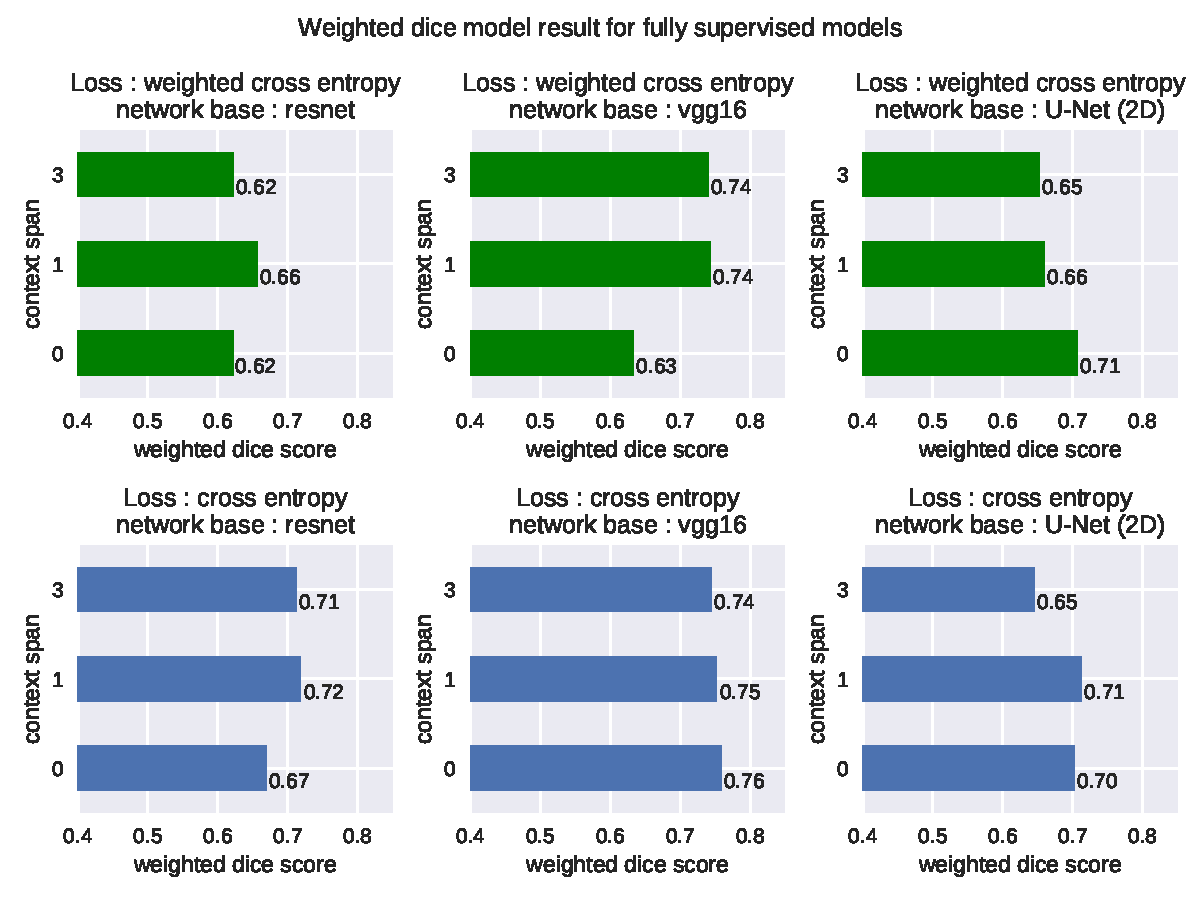
\includegraphics[width=.98\textwidth]{images/FullySupervised.pdf}
    \caption{Results of the fully supervised experiments.
    The indicated model performance metrics are calculated on the test set.
    The columns represent de weighted dice scores for models based on the same network architecture with different loss functions.
    \label{fig:referenceExperiments}}
\end{SCfigure}

\begin{SCfigure}[][htb]
    \centering
    \begin{minipage}{.98\textwidth}
        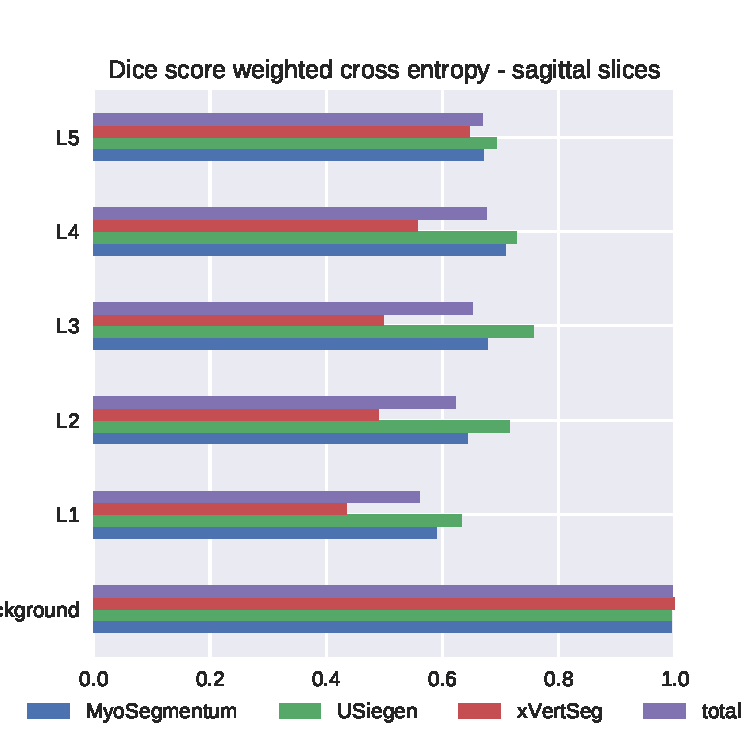
\includegraphics[width=.98\textwidth]{images/full_perClass_perSource_weighted.pdf}
    \end{minipage} 
    \begin{minipage}{0.98\textwidth}
        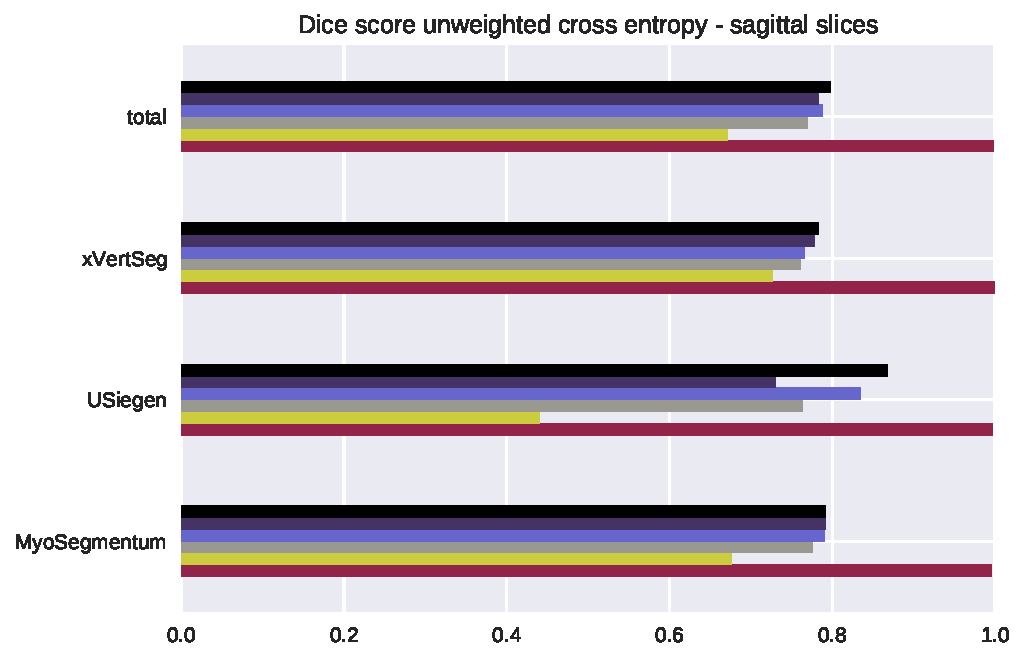
\includegraphics[width=.98\textwidth]{images/full_perClass_perSource_notweighted.pdf}
    \end{minipage}
    \caption{Detailed result for the fully supervised model trained without context slices and with a weighted cross entropy loss function.
    The model trained with the unweighted loss performs better than the result shown in figure \ref{fig:referenceWeighted} for the weighted cross entropy loss function.
    \label{fig:referenceWeighted} 
    }
\end{SCfigure}

\section{Conclusion}
\par{
    Based on the results shown in figure \ref{fig:referenceExperiments}, it was decided to perform the weakly supervised experiments with the model based on VGG16 FCN8 with one context slice.
    The reference performance metric to compare experiments with models trained on weakly supervised data is $\text{Dice}_{wi}=0,76$.
}




\chapter{Single dimension experiments \label{sec:singleDimension}}

\par{
    This chapter discusses the results of several experiments in the construction of single-dimensional models.
    The objective of these experiments is to investigate the influence different model hyperparameters have on the model performance.
    Based on this investigation, the hyperparameters for the single-dimensional models in the final step can be chosen.  
}

\section{Single dimension weakly supervised models}

\par{
    In this section, the results of experiments with different model hyperparameters are compared to each other.
    The point annotation sets are generated from the available full annotation masks for each slice.
    In this work, different datasets were used with different levels of provided annotation. 
    Annotation differences between different datasets are listed in table \ref{tab:datasetReferences} on page \pageref{tab:datasetReferences}.
}
\par{
    For three datasets\footnote{The three datasets for which complete annotation is available are the xVertSeg dataset, the UniSiegen dataset and the MyoSegmentum dataset. Of which the MyoSegmentum dataset is the largest by far.},
    full annotation masks are available, meaning that these scan volumes are labelled with volumes for each of the five lumbar vertebrae.
    For each voxel, the ground truth indicates whether it belongs to a lumbar vertebra and which vertebra.
    For one dataset (PLoS), only semantic segmentation is available. It means that the lumbar vertebrae are indicated as one class but not distinguished. 
    With each voxel in the PLoS dataset, ground truth is associated that indicates if it belongs to a lumbar vertebra. There is no label, however, to indicate which of the lumbar vertebrae this is.
}
\par{
    When a scan is sliced along the craniocaudal axis\footnote{
        The nomenclature of anatomical planes and axis is illustrated in figure \ref{fig:anatomicalPlains} on page \pageref{fig:anatomicalPlains}.
        The craniocaudal axis is the vertical axis when the patient is standing up.} 
    a human can distinguish all 5 lumbar vertebrae (after some practice).
    Therefore, one may hope the single-dimension models trained on sagittal or frontal slices will be able to do the same.
    Even though delineating a vertebra on a transverse slice is possible, identifying which vertebra is presented is challenging for a human.
    Supported by a brief test, it was confirmed that trying to estimate 5 vertebra classes from the transverse slices only provides very confusing results.
    The models trained on the transverse slices only intend to label the slice pixels as either background (0) or vertebra (1), 
    whereas the models trained on the sagittal and frontal slices intend to indicate which of 6 classes\footnote{0 for background, 1 for $L1$, 2 for $L2$, 3 for $L3$, 4 for $L4$ and 5 for $L2$} the pixel belongs to.
}
\par{
    The models trained to segment sagittal and frontal slices were trained on datasets xVertSeg, UniSiegen and MyoSegmenTUM.
    From the available full masks, point annotation labels were extracted.
    The models trained to segment transverse slices\footnote{This segmentation is, as stated not based on distinguishing separate lumbar vertebrae from each other.} 
    are trained on the same three datasets and additionally on the PLoS dataset.    
}
\par{
    The model performance results are compared based on the weighted dice score calculated on the test set.
    This metric is described in chapter \ref{sec:dice} on page \pageref{sec:dice}.
}


\subsection{Evaluation of the model Hyperparameters}

\par{
    To obtain the best model hyperparameters to train the single-dimension models, several tests were conducted to estimate the influence of model components and model hyperparameters\footnote{
        One could argue that the number of annotation points is not a \textit{model} hyperparameter. It is an essential parameter for the \textit{modelling} approach in general.
    } on the model performance.
}

\subsubsection{Weighted vs unweighted point loss performance}

\par{
    Equation \ref{eq:LP} on page \pageref{eq:LP} defines the point loss $\mathcal{L}_P$. 
    In this equation, the factor $w_{\mathcal{Y}_i(\vec{p})}$ indicates a weight that can be assigned to each of the output classes.
    Since data classes can be unbalanced, these weights can help to counter this imbalance.
    In this problem (based on the available datasets), there are about 500 times more background voxels than voxels belonging to a lumbar vertebra.
    By weighing with a factor proportional\footnote{The weighting vector is normalized.} to this ratio, this imbalance can be countered\footnote{
        When full data labels are available, the counts of the voxel types are available for the train set (one should not include the counts of the validation \& test set to avoid data leakage).
        In principle, this information is not necessarily available when only point level annotation is available. In this work, it is considered that (at least an approximation) of the ratios can be available as prior knowledge.
    }. In the unweighted case, $w_{\cdot} = 1$.
}
\par{
    In figure \ref{fig:weighted_vs_unweighted}, the difference between the weighted dice score \& the average dice score on the test set is compared for two models trained on the transverse slices.
    This result shows that the result of the non-weighted segmentation is better than the result of the model trained with weighted loss.
    Contrary to fully supervised models, in the weakly supervised case, the ratio between \textit{labelled} points is not as unbalanced as the ratio between the actual class pixels in the result.
    This explains the weighted point loss performance compared to the unweighted point loss performance.
    An approach that is not tested in this work is to weigh proportional to the inverse of the number of \textit{annotation} points per class instead of weighing proportional to the number of \textit{ground truth} pixels.
}


\begin{SCfigure}[][htb]
    \centering
    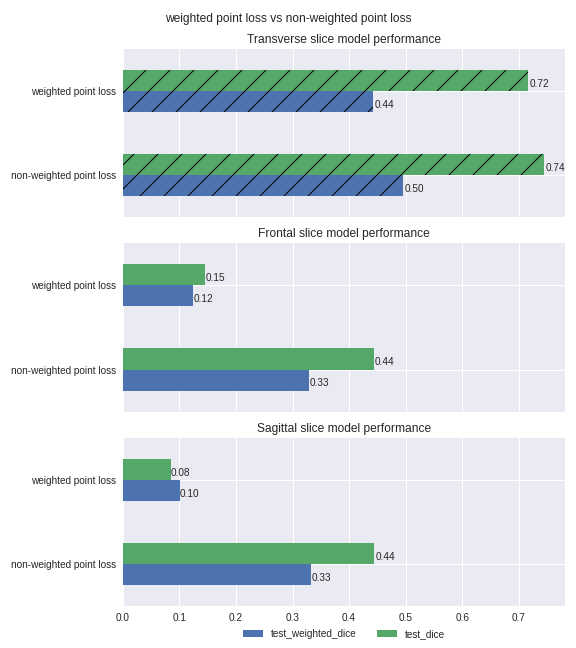
\includegraphics[width=.95\textwidth]{images/weightedvsnonweighted.png}
    \caption{Illustration of the difference in model performance between a weighted point loss function and the unweighted point loss function\label{fig:weighted_vs_unweighted}}
\end{SCfigure}

\subsubsection{Value of the added loss components}
\par{
    In this work, two-loss components were added to the consistency loss published in \cite{Laradji}.
    
    Where \cite{Laradji} is based only on the point loss $\mathcal{L}_P$ and the consistency loss $\mathcal{L}_C$, this work makes use of two extra loss components:
    the prior extend loss $\mathcal{L}_E$ and the separation loss $\mathcal{L}_S$. The four-loss components used in this work are described in more detail in \ref{sec:LossFunctions}.
    Figure \ref{fig:addedLossComponents} shows experimental results validating the positive influence these added loss terms have on the model performance.
}


\begin{SCfigure}[][htb]
    \centering
    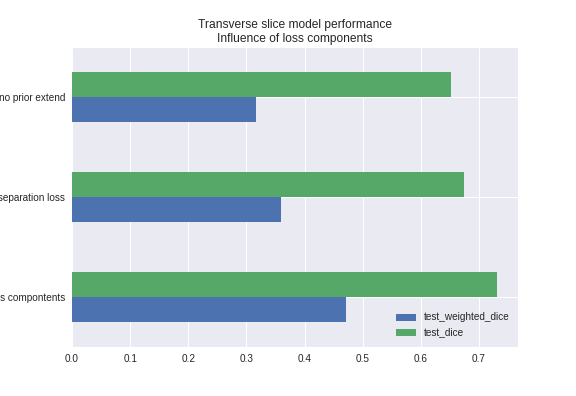
\includegraphics[width=.95\textwidth]{images/TransverseModel_Losscomponents.png}
    \caption{Evaluation of the added value of loss components. \label{fig:addedLossComponents}}
\end{SCfigure}

\subsection{Evolution of the model performance with increased labelling effort}
\par{
    The most basic modelling hyperparameter for a point annotation modelling campaign is the number of labelling points one asks the expert to provide.
    This section presents experimental results to estimate the influence of the number of annotation points on the resulting model performance.
    Intuitively, one would expect the model performance to increase with the number of annotation points provided.
    This hypothesis turns out to be false.
}
\begin{SCfigure}[][htb]
    \centering
    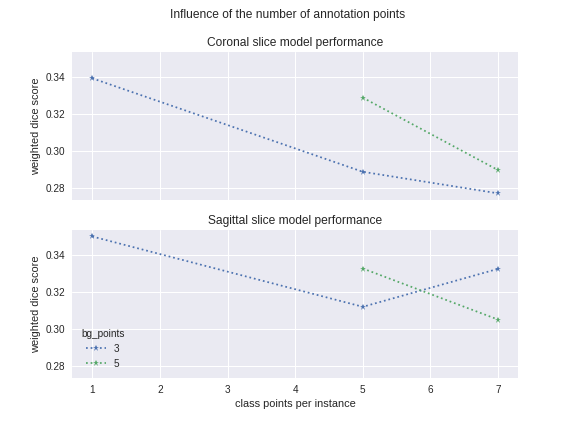
\includegraphics[width=.95\textwidth]{images/BlobPoints_influence.png}
    \caption{Evaluation of the added value of loss components. \label{fig:addedLossComponents}}
\end{SCfigure}
\par{
    Figure \ref{fig:addedLossComponents} shows the weighted dice score actually decreases with more annotation points.
    This is caused by the increased recall of the model. 
    The model becomes very eager to find class points, this causes a lot of background pixels to be wrongly classified as class points.
    The resulting decrease in precision causes the F1 score to decrease.
}
\todo[inline]{Werk verder uit met afbeelding en tabel}



\chapter{Single dimension model combination\label{sec:combination}}

All models are designed for $352 \times 352$ crops of the 2D slices.
The estimation of the slice is obtained by combining the model estimations on all crops taken from this slice.

\section{Volume combination procedure}

Combining the results of three different single dimension models is performed in two steps:
\begin{enumerate}
    \item The resulting classification volumes are first combined with a rule-based method
    \item After this rule-based combination, the resulting segmentation estimation is smoothened with a morphological filter.
\end{enumerate}

\subsection{Rule based result combination}
Three single dimension models are trained:
\begin{description}
    \item[Transverse slices] offer little context to indicate which of the lumbar vertebrae they contain. 
    It does not seem easy even for a human expert to indicate which vertebra is visible on the slice.
    The model trained on these slices is intended only for semantic segmentation.
    Each pixel is inferred only if it represents a vertebra, without distinction between the different lumbar vertebrae. 
    \item[Sagittal \& Coronal slices] do offer the necessary context to distinguish between $L_1$ to $L_5$. 
    The models trained on these slices do indicate the specific lumbar vertebra index. 
\end{description}

Based on the observation that all trained models accurately predict the background, these three models are combined in a straightforward way\footnote{
    The resulting estimations from a model for an input volume is again a three-dimensional volume ($\in \mathbb{N}^3$) with the same dimensions.
}.

\begin{algorithm}[H]
    \SetAlgoLined
    \KwData{
        Results $y_.$ of three models indicating an estimated class for all positions $\vec{p}$ in the volume.
        \begin{itemize} 
            \item Transverse model $y_t \in \mathbb{N}^3: \forall y_t(\vec{p}) \in \{ 0, 1 \}$
            \item Sagittal model $y_s \in \mathbb{N}^3: \forall y_t(\vec{p}) \in \{ 0, 1, 2, 3, 4, 5 \}$ 
            \item Coronal model $y_c \in \mathbb{N}^3: \forall y_t(\vec{p}) \in \{ 0, 1, 2, 3, 4, 5 \}$ 
        \end{itemize}
    }
    \KwResult{Combination of the three model results $y_f$.}
    \For{all $\vec{p}$}{
        \eIf{$y_t[\vec{p}] = 1 \wedge y_s[\vec{p}] = y_c[\vec{p}]$}{
            $y_f[\vec{p}] \leftarrow y_s[\vec{p}]$ \;
        }{
            $y_f[\vec{p}] \leftarrow 0$ \;
        }
    }
   \caption{Rule based combination of model results from three single dimension models}
\end{algorithm}

\todo[inline]{Image illustrating the combination}

\subsection{Morphological smoothing}
After the rule-based combination of estimations from different single dimension models, the result is smoothened with standard morphological filters.
These filters are combinations of the morphological \textit{erosion} and \textit{dilation} operators.
\todo[inline]{How deep should these morphological filters be discussed?}
\begin{itemize}
    \item Possible noise is suppressed by first opening and then closing the volumes.
    \item The estimated volumes are observed to overestimate the extent of the vertebrae. For this reason, an erosion step is performed to decrease the overall extent of the class masks.
\end{itemize}

The procedure mentioned above has two Hyperparameters: the number of iterations for the denoising filters and the number of iterations for the erosion filter.
Both hyperparameters are estimated by calculating the same evaluation metric, the weigh dice score on the validation set, as for the single-dimensional model evaluation. 


\begin{SCfigure}[][htb]
    \centering
    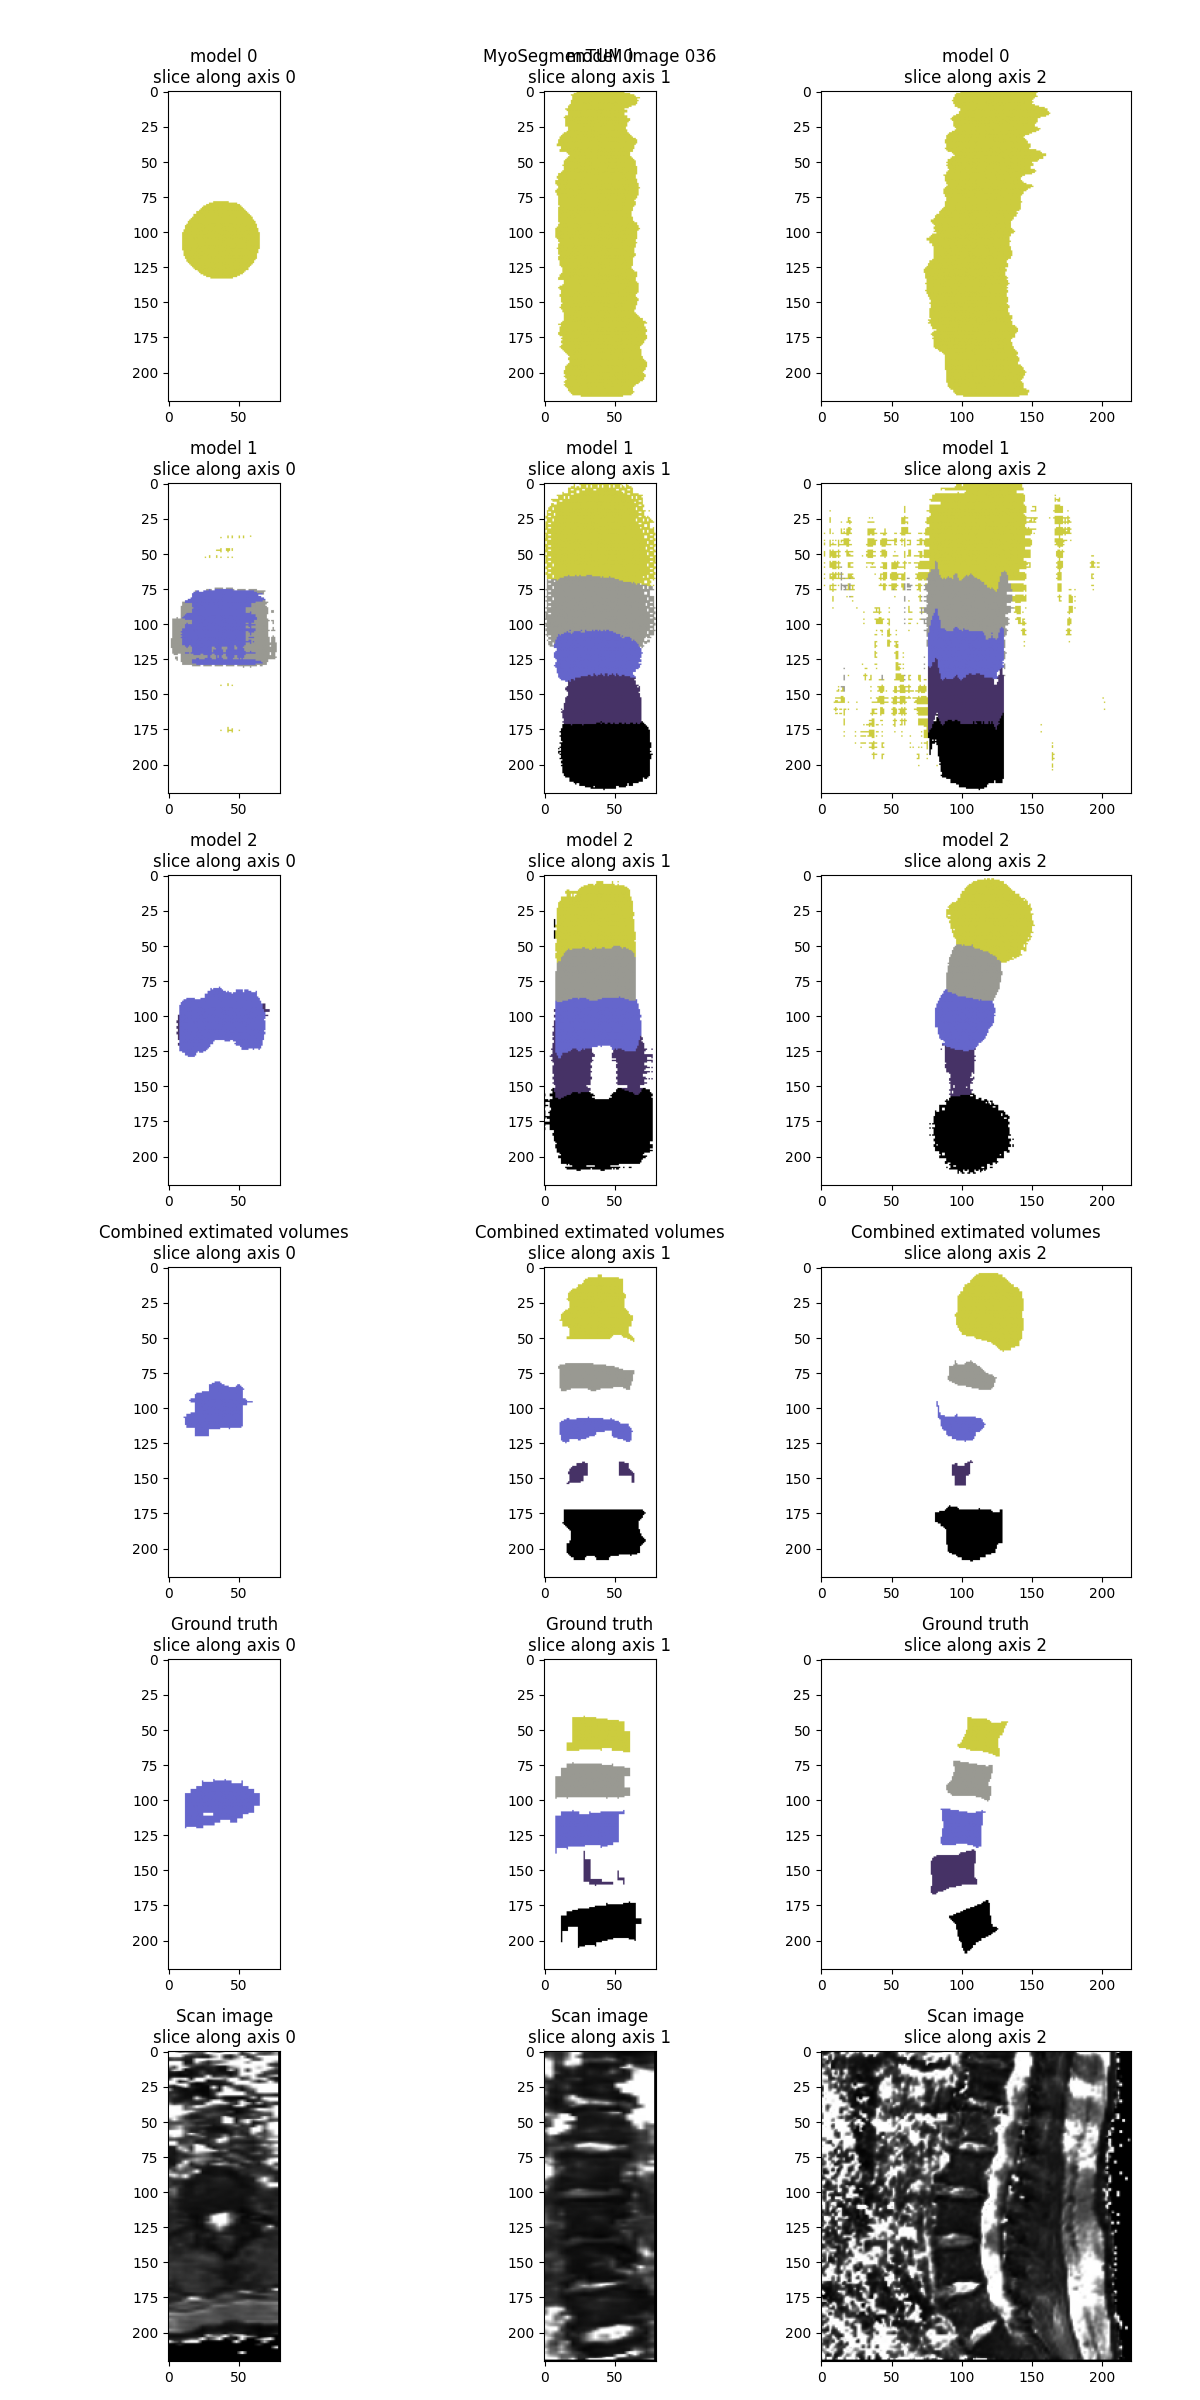
\includegraphics[width=.95\textwidth]{images/morphmask_denoise1_erode1_MyoSegmenTUM_036.png}
    \caption{
        Result of the combination of the three single dimension model results for volume MyoSegmenTUM nr 43.
        The colours indicate the vertebra classes. Only one semantic class is estimated in the first row, illustrating the model trained on transversal slices.
        On the first three rows, slices of the resulting segmentations from the single dimension models are shown. 
        It is clear these masks contain some artefacts and are not always in agreement with each other.
        On the fourth row, the result after mask combination and morphological smoothing is shown. 
        This corresponds more closely to the ground truth mask, shown on the fifth row.
        This final mask, shown on the fourth row, will be used as a pseudo mask to approximate the unknown ground truth mask.
        In the last row, the corresponding images are shown.
    }
\end{SCfigure}

\section{Pseudo mask performance}

\chapter{Pseudo mask training}

Time to evaluate
performance

\newgeometry{total={210mm,297mm},left=20mm,right=20mm,bindingoffset=5mm, top=25mm,bottom=25mm} 
\begin{partwithabstract}{Conclusions}
    This part of the document summarizes the most important conclusions from this work and possible ideas as a way forward after this work.
    The part starts with an evaluation and discussion of the labelling cost necessary to make the final model. 
    Finally, the lessons learned from this project are laid out and some ideas for further development of weakly supervised models for medical applications are presented. 
\end{partwithabstract}
\restoregeometry

\chapter{Conclusions}

\chapter{Remarks for future work}

\begin{enumerate}
    \item Finer prior extrend: per vertebra, per direction
    \item Dig deeper in the difference between datasets
    \item Dig deeper how weighted loss might help - Is oversampling a better idea?
\end{enumerate}

\appendix

\newgeometry{total={210mm,297mm},left=30mm,right=30mm,bindingoffset=5mm, top=25mm,bottom=25mm}
\begin{partwithabstract}{Appendix}
  Apendices to the document:
  \begin{enumerate}
    \item Software environment used
    \item Agreement documents for use of two datasets.
  \end{enumerate}
\end{partwithabstract}
\restoregeometry

\chapter{Train test split detail\label{sec:appendix_split}}

The datasets in this research are both stratified and grouped (due to USiegen containing multiple scans from the same patient).
These were splitted in a train, validation and test set taking into account these characteristics.
This was discussed in chapter \ref{sec:trainValTestSplit} on page \pageref{sec:trainValTestSplit}.
The result of this operation is detailed in the following tables.

\begin{tabular}{llll}
\toprule
{} &           patient &           scan\_id &  split \\
\midrule
0   &  MyoSegmenTUM\_001 &  MyoSegmenTUM\_001 &  train \\
1   &  MyoSegmenTUM\_002 &  MyoSegmenTUM\_002 &   test \\
2   &  MyoSegmenTUM\_003 &  MyoSegmenTUM\_003 &  train \\
3   &  MyoSegmenTUM\_004 &  MyoSegmenTUM\_004 &  train \\
4   &  MyoSegmenTUM\_005 &  MyoSegmenTUM\_005 &   xval \\
5   &  MyoSegmenTUM\_006 &  MyoSegmenTUM\_006 &   test \\
6   &  MyoSegmenTUM\_007 &  MyoSegmenTUM\_007 &  train \\
7   &  MyoSegmenTUM\_008 &  MyoSegmenTUM\_008 &  train \\
8   &  MyoSegmenTUM\_009 &  MyoSegmenTUM\_009 &  train \\
9   &  MyoSegmenTUM\_010 &  MyoSegmenTUM\_010 &  train \\
10  &  MyoSegmenTUM\_011 &  MyoSegmenTUM\_011 &   test \\
11  &  MyoSegmenTUM\_012 &  MyoSegmenTUM\_012 &   test \\
12  &  MyoSegmenTUM\_013 &  MyoSegmenTUM\_013 &  train \\
13  &  MyoSegmenTUM\_014 &  MyoSegmenTUM\_014 &  train \\
14  &  MyoSegmenTUM\_015 &  MyoSegmenTUM\_015 &  train \\
15  &  MyoSegmenTUM\_016 &  MyoSegmenTUM\_016 &   xval \\
16  &  MyoSegmenTUM\_017 &  MyoSegmenTUM\_017 &  train \\
17  &  MyoSegmenTUM\_018 &  MyoSegmenTUM\_018 &  train \\
18  &  MyoSegmenTUM\_019 &  MyoSegmenTUM\_019 &   xval \\
19  &  MyoSegmenTUM\_020 &  MyoSegmenTUM\_020 &  train \\
20  &  MyoSegmenTUM\_021 &  MyoSegmenTUM\_021 &  train \\
21  &  MyoSegmenTUM\_022 &  MyoSegmenTUM\_022 &   test \\
22  &  MyoSegmenTUM\_023 &  MyoSegmenTUM\_023 &  train \\
23  &  MyoSegmenTUM\_024 &  MyoSegmenTUM\_024 &   test \\
24  &  MyoSegmenTUM\_025 &  MyoSegmenTUM\_025 &  train \\
25  &  MyoSegmenTUM\_026 &  MyoSegmenTUM\_026 &  train \\
26  &  MyoSegmenTUM\_027 &  MyoSegmenTUM\_027 &  train \\
27  &  MyoSegmenTUM\_028 &  MyoSegmenTUM\_028 &   xval \\
28  &  MyoSegmenTUM\_029 &  MyoSegmenTUM\_029 &  train \\
29  &  MyoSegmenTUM\_030 &  MyoSegmenTUM\_030 &  train \\
30  &  MyoSegmenTUM\_031 &  MyoSegmenTUM\_031 &   xval \\
31  &  MyoSegmenTUM\_032 &  MyoSegmenTUM\_032 &  train \\
32  &  MyoSegmenTUM\_034 &  MyoSegmenTUM\_034 &  train \\
33  &  MyoSegmenTUM\_035 &  MyoSegmenTUM\_035 &   test \\
34  &  MyoSegmenTUM\_036 &  MyoSegmenTUM\_036 &   xval \\
35  &  MyoSegmenTUM\_037 &  MyoSegmenTUM\_037 &   xval \\
36  &  MyoSegmenTUM\_038 &  MyoSegmenTUM\_038 &  train \\
37  &  MyoSegmenTUM\_039 &  MyoSegmenTUM\_039 &  train \\
38  &  MyoSegmenTUM\_040 &  MyoSegmenTUM\_040 &  train \\
39  &  MyoSegmenTUM\_041 &  MyoSegmenTUM\_041 &  train \\
40  &  MyoSegmenTUM\_042 &  MyoSegmenTUM\_042 &  train \\
41  &  MyoSegmenTUM\_043 &  MyoSegmenTUM\_043 &   xval \\
42  &  MyoSegmenTUM\_044 &  MyoSegmenTUM\_044 &  train \\
43  &  MyoSegmenTUM\_045 &  MyoSegmenTUM\_045 &  train \\
44  &  MyoSegmenTUM\_046 &  MyoSegmenTUM\_046 &  train \\
45  &  MyoSegmenTUM\_047 &  MyoSegmenTUM\_047 &  train \\
46  &  MyoSegmenTUM\_048 &  MyoSegmenTUM\_048 &  train \\
47  &  MyoSegmenTUM\_049 &  MyoSegmenTUM\_049 &   test \\
48  &  MyoSegmenTUM\_050 &  MyoSegmenTUM\_050 &  train \\
49  &  MyoSegmenTUM\_051 &  MyoSegmenTUM\_051 &   test \\
50  &  MyoSegmenTUM\_052 &  MyoSegmenTUM\_052 &   xval \\
51  &          PLoS\_001 &          PLoS\_001 &  train \\
52  &          PLoS\_002 &          PLoS\_002 &  train \\
53  &          PLoS\_003 &          PLoS\_003 &  train \\
54  &          PLoS\_004 &          PLoS\_004 &  train \\
55  &          PLoS\_005 &          PLoS\_005 &   xval \\
56  &          PLoS\_006 &          PLoS\_006 &   test \\
57  &          PLoS\_007 &          PLoS\_007 &  train \\
58  &          PLoS\_008 &          PLoS\_008 &  train \\
59  &          PLoS\_009 &          PLoS\_009 &  train \\
60  &          PLoS\_010 &          PLoS\_010 &  train \\
61  &          PLoS\_011 &          PLoS\_011 &   xval \\
62  &          PLoS\_012 &          PLoS\_012 &   test \\
63  &          PLoS\_013 &          PLoS\_013 &  train \\
64  &          PLoS\_014 &          PLoS\_014 &  train \\
65  &          PLoS\_015 &          PLoS\_015 &  train \\
66  &          PLoS\_016 &          PLoS\_016 &  train \\
67  &          PLoS\_017 &          PLoS\_017 &   xval \\
68  &          PLoS\_018 &          PLoS\_018 &   test \\
69  &          PLoS\_019 &          PLoS\_019 &  train \\
70  &          PLoS\_020 &          PLoS\_020 &  train \\
71  &          PLoS\_021 &          PLoS\_021 &   xval \\
72  &          PLoS\_022 &          PLoS\_022 &   test \\
73  &       USiegen\_001 &       USiegen\_003 &  train \\
74  &       USiegen\_001 &       USiegen\_006 &  train \\
75  &       USiegen\_001 &       USiegen\_016 &  train \\
76  &       USiegen\_002 &       USiegen\_008 &  train \\
77  &       USiegen\_002 &       USiegen\_014 &  train \\
78  &       USiegen\_002 &       USiegen\_001 &  train \\
79  &       USiegen\_002 &       USiegen\_010 &  train \\
80  &       USiegen\_002 &       USiegen\_000 &  train \\
81  &       USiegen\_004 &       USiegen\_002 &  train \\
82  &       USiegen\_007 &       USiegen\_005 &  train \\
83  &       USiegen\_007 &       USiegen\_009 &  train \\
84  &       USiegen\_008 &       USiegen\_012 &   test \\
85  &       USiegen\_009 &       USiegen\_015 &  train \\
86  &       USiegen\_010 &       USiegen\_004 &   xval \\
87  &       USiegen\_015 &       USiegen\_007 &  train \\
88  &       USiegen\_016 &       USiegen\_013 &  train \\
89  &       USiegen\_018 &       USiegen\_011 &   test \\
90  &      xVertSeg\_001 &      xVertSeg\_001 &  train \\
91  &      xVertSeg\_002 &      xVertSeg\_002 &  train \\
92  &      xVertSeg\_003 &      xVertSeg\_003 &  train \\
93  &      xVertSeg\_004 &      xVertSeg\_004 &  train \\
94  &      xVertSeg\_005 &      xVertSeg\_005 &  train \\
95  &      xVertSeg\_006 &      xVertSeg\_006 &  train \\
96  &      xVertSeg\_007 &      xVertSeg\_007 &   xval \\
97  &      xVertSeg\_008 &      xVertSeg\_008 &  train \\
98  &      xVertSeg\_009 &      xVertSeg\_009 &   xval \\
99  &      xVertSeg\_010 &      xVertSeg\_010 &  train \\
100 &      xVertSeg\_011 &      xVertSeg\_011 &   test \\
101 &      xVertSeg\_012 &      xVertSeg\_012 &  train \\
102 &      xVertSeg\_013 &      xVertSeg\_013 &  train \\
103 &      xVertSeg\_014 &      xVertSeg\_014 &   test \\
104 &      xVertSeg\_015 &      xVertSeg\_015 &   xval \\
\bottomrule
\end{tabular}



\chapter{Used software \& Reproducability of this research}

\section{Reproducability of the used environment}
The reproducability of this work has been ensured in several ways:
\begin{description}
  \item[Data]: All datasets used in this project are publically available. For some datasets, it is required to request permission, like the author of this work has done.
  \item[Software]: This project was performed completely in python, a publically available programming language. 
  All packages used are open-source.
  To reproduce this research, no software has to be purchased. 
  \item[Code]: Both code an text of this project can be found on a public \texttt{GitHub} repository: \url{https://github.com/JanAlexanderPersonal/MastatThesis.git}.
  \footnote{It is possible that small adaptations of the code are required to run it on other hardware. For example, to run it using a GPU with less internal memory it could be necessary to reduce the batch size.}. 
  \item[Docker]: The specific environment to run the code mentioned above can also be found in the mentioned GitHub repository in the form a dockerfile.
  It should be noted that this dockerfile requires a GPU that supports CUDA.   
\end{description}

The above mentioned aspects should allow other researchers to reproduce the results in this document.
This work makes use of parts of \textit{haven.ai} \footnote{This is a collection of libraries developed by the team of dr. I. Laradji to manage different experiments in deep learning research.} 
as a basis to manage different experiments.
These experiments are conducted using the deep learning library \textit{PyTorch}.
This tool is widely used in boty industry and academic research.
A list of other Machine Learning tools used in this work is provided below.
Table \ref{tab:UsedTools} is not an exhaustive list of all  python libraries used in this work.
It aims to list the more advanced tools, crucial for this work.

\begin{SCtable}[\sidecaptionrelwidth][h]
 
  \begin{tabular}{ p{2cm} l l } 
   \hline
   \hline
   \textbf{Library} & \textbf{version} & \textbf{reference}    \\
   \hline 
  Python & 3.8 & Programming language \\
   \hline
   \multicolumn{3}{c}{Deep learning and machine learning tools} \\
   \hline
   PyTorch & 1.7.1 & Deep learning library \\ 
   scikit-learn & 0.24.2 & Machine learning toolbox \\
   \hline
   \multicolumn{3}{c}{Tools to work with (medical) images} \\
   \hline
   SimpleITK & 2.0.2 & Library for medical images \\ 
   kornia & 0.2.0 & Computer vision library linked to torch \\
   scikit-image & 0.18.1 & Image manipulation library \\
   Pillow & 8.2.0 & Image manipulation\\
   \hline
   \multicolumn{3}{c}{Tools for matrix \& scientific computation} \\
   \hline
   numpy & 1.20.3 & matrix manipulation \\
   scipy & 1.6.3 & scientific calculation \\
   \hline
   \multicolumn{3}{c}{Result visualization} \\
   \hline
   matplotlib & 3.4.2 & data visualization \\ 
   seaborn & 0.11.1 & data visualization \\
   \multicolumn{3}{c}{Neural network experiment management} \\
   \hline
   haven &  & experiment management \\ 
   \hline
   \hline
  \end{tabular}
  \caption{Python libraries used. \label{tab:UsedTools}}

\end{SCtable}

Table \ref{tab:UsedTools} is not an exhaustive list of all libraries used in this work.
One can quickly dublicate the environment used in this work by building the \textit{Docker} environment defined in \texttt{dockerfiles} (part of the \texttt{GitHub} repository).

\section{Hardware\label{sec:hardware}}
The main hardware components of the device used for this work are listed below:

Intel® Core™ i7-9700 CPU @ 3.00GHz $\times$ 8 \\
RAM : 32 GB

\textsc{GPU}:\\
\hspace{5mm}GeForce RTX 2080 Ti (4352 CUDA cores)\\
\hspace{5mm}total memory 11264 MB\\
\hspace{5mm}CUDA version 11.2



\section{Other}
The formatting of this document, bringing Tufte layout elements in the \LaTeX{} memoir class, is based on the excelent post found on \url{https://tex.stackexchange.com/questions/275565/tufte-layout-in-painless-memoir}.
Didier Dufragne gave a few very helpful tips for improving this layout.
The Neural network architecture illustrations were made using this project: \url{https://github.com/HarisIqbal88/PlotNeuralNet}.
The conceptual illustration of the neural network idea on page \pageref{fig:ann} is based on \url{https://tex.stackexchange.com/questions/153957/drawing-neural-network-with-tikz}.



\newgeometry{total={210mm,297mm},left=30mm,right=30mm,bindingoffset=5mm, top=25mm,bottom=25mm}
\chapter{Dataset agreements\label{seg:datasetagreement}}


\includegraphics[width=17cm]{/home/thesis/images/AgreementxVertSeg.png}

\chapter{Predefence and seminars}
\par{
  On March 31$^st$, 2021 the concept of this work was presented in a poster session seated by Prof. Stijn Vansteelandt.
The poster used during this event is included on the next page for reference.
}




\includepdf[fitpaper=true, pages=-]{/home/thesis/images/Addendum_thesis_seminars.pdf}
\includepdf[fitpaper=true, pages=-]{/home/thesis/images/Poster_JanAlexander.pdf}


%\nocite{*} 
\printbibliography

\end{document}

